% interactcadsample.tex
%DIF LATEXDIFF DIFFERENCE FILE
%DIF DEL paper-submission2.tex   Tue Apr 14 09:38:37 2026
%DIF ADD paper.tex               Fri Jul 10 06:42:48 2026
% v1.04 - May 2023

\documentclass[]{interact}

\usepackage{epstopdf}% To incorporate .eps illustrations using PDFLaTeX, etc.
\usepackage{subfigure}% Support for small, `sub' figures and tables
%\usepackage[nolists,tablesfirst]{endfloat}% To `separate' figures and tables from text if required

\usepackage{natbib}% Citation support using natbib.sty
\bibpunct[, ]{(}{)}{;}{a}{}{,}% Citation support using natbib.sty
\renewcommand\bibfont{\fontsize{10}{12}\selectfont}% Bibliography support using natbib.sty

\theoremstyle{plain}% Theorem-like structures provided by amsthm.sty
\newtheorem{theorem}{Theorem}[section]
\newtheorem{lemma}[theorem]{Lemma}
\newtheorem{corollary}[theorem]{Corollary}
\newtheorem{proposition}[theorem]{Proposition}

\theoremstyle{definition}
\newtheorem{definition}[theorem]{Definition}
\newtheorem{example}[theorem]{Example}

\theoremstyle{remark}
\newtheorem{remark}{Remark}
\newtheorem{notation}{Notation}


% tightlist command for lists without linebreak
\providecommand{\tightlist}{%
  \setlength{\itemsep}{0pt}\setlength{\parskip}{0pt}}



\usepackage{lscape}
\usepackage{hyperref}
\usepackage[utf8]{inputenc}
\def\tightlist{}
\usepackage{setspace}
\doublespacing

\usepackage{booktabs}
\usepackage{longtable}
\usepackage{array}
\usepackage{multirow}
\usepackage{wrapfig}
\usepackage{float}
\usepackage{colortbl}
\usepackage{pdflscape}
\usepackage{tabu}
\usepackage{threeparttable}
\usepackage{threeparttablex}
\usepackage[normalem]{ulem}
\usepackage{makecell}
\usepackage{xcolor}
%DIF PREAMBLE EXTENSION ADDED BY LATEXDIFF
%DIF UNDERLINE PREAMBLE %DIF PREAMBLE
\RequirePackage[normalem]{ulem} %DIF PREAMBLE
\RequirePackage{color}\definecolor{RED}{rgb}{1,0,0}\definecolor{BLUE}{rgb}{0,0,1} %DIF PREAMBLE
\providecommand{\DIFaddtex}[1]{{\protect\color{blue}\uwave{#1}}} %DIF PREAMBLE
\providecommand{\DIFdeltex}[1]{{\protect\color{red}\sout{#1}}}                      %DIF PREAMBLE
%DIF SAFE PREAMBLE %DIF PREAMBLE
\providecommand{\DIFaddbegin}{} %DIF PREAMBLE
\providecommand{\DIFaddend}{} %DIF PREAMBLE
\providecommand{\DIFdelbegin}{} %DIF PREAMBLE
\providecommand{\DIFdelend}{} %DIF PREAMBLE
\providecommand{\DIFmodbegin}{} %DIF PREAMBLE
\providecommand{\DIFmodend}{} %DIF PREAMBLE
%DIF FLOATSAFE PREAMBLE %DIF PREAMBLE
\providecommand{\DIFaddFL}[1]{\DIFadd{#1}} %DIF PREAMBLE
\providecommand{\DIFdelFL}[1]{\DIFdel{#1}} %DIF PREAMBLE
\providecommand{\DIFaddbeginFL}{} %DIF PREAMBLE
\providecommand{\DIFaddendFL}{} %DIF PREAMBLE
\providecommand{\DIFdelbeginFL}{} %DIF PREAMBLE
\providecommand{\DIFdelendFL}{} %DIF PREAMBLE
%DIF HYPERREF PREAMBLE %DIF PREAMBLE
\providecommand{\DIFadd}[1]{\texorpdfstring{\DIFaddtex{#1}}{#1}} %DIF PREAMBLE
\providecommand{\DIFdel}[1]{\texorpdfstring{\DIFdeltex{#1}}{}} %DIF PREAMBLE
%DIF COLORLISTINGS PREAMBLE %DIF PREAMBLE
\RequirePackage{listings} %DIF PREAMBLE
\RequirePackage{color} %DIF PREAMBLE
\lstdefinelanguage{DIFcode}{ %DIF PREAMBLE
%DIF DIFCODE_UNDERLINE %DIF PREAMBLE
  moredelim=[il][\color{red}\sout]{\%DIF\ <\ }, %DIF PREAMBLE
  moredelim=[il][\color{blue}\uwave]{\%DIF\ >\ } %DIF PREAMBLE
} %DIF PREAMBLE
\lstdefinestyle{DIFverbatimstyle}{ %DIF PREAMBLE
	language=DIFcode, %DIF PREAMBLE
	basicstyle=\ttfamily, %DIF PREAMBLE
	columns=fullflexible, %DIF PREAMBLE
	keepspaces=true %DIF PREAMBLE
} %DIF PREAMBLE
\lstnewenvironment{DIFverbatim}{\lstset{style=DIFverbatimstyle}}{} %DIF PREAMBLE
\lstnewenvironment{DIFverbatim*}{\lstset{style=DIFverbatimstyle,showspaces=true}}{} %DIF PREAMBLE
%DIF END PREAMBLE EXTENSION ADDED BY LATEXDIFF

\begin{document}


\articletype{}

\title{Automated Assessment of Residual Plots with Computer Vision
Models}


\author{\name{Weihao Li$^{a, b}$, Dianne Cook$^{a}$, Emi
Tanaka$^{b}$, Susan VanderPlas$^{c}$, Klaus Ackermann$^{a}$}
\affil{$^{a}$Department of Econometrics and Business Statistics, Monash
University, Clayton, VIC, Australia; $^{b}$Research School of Finance,
Actuarial Studies and Statistics, Australian National University, Acton,
ACT, Australia; $^{c}$Department of Statistics, University of Nebraska,
Lincoln, Nebraska, USA}
}


\maketitle

\begin{abstract}
Plotting the residuals is a recommended procedure to diagnose deviations
from linear model assumptions, such as non-linearity,
heteroskedasticity, and non-normality. The presence of structure in
residual plots can be tested using the lineup protocol to do visual
inference. There are a variety of conventional residual tests, but the
lineup protocol, used as a statistical test, performs better for
diagnostic purposes because it is less sensitive and applies more
broadly to different types of departures. However, the lineup protocol
relies on human judgment which limits its scalability. This work
presents a solution by providing a computer vision model to automate the
assessment of residual plots. It is trained to predict a distance
measure that quantifies the disparity between the residual distribution
of a fitted classical normal linear regression model and the reference
distribution, based on Kullback-Leibler divergence. Evaluation using
data from a prior human-subject experiment shows the model exhibits
lower sensitivity than conventional tests but higher sensitivity than
human visual tests. Several examples from classical papers and
contemporary data demonstrate the method's practical utility in
automating residual diagnostics.
\end{abstract}

\begin{keywords}
statistical graphics; data visualization; visual inference; computer
vision; machine learning; hypothesis testing; regression analysis;
cognitive perception; simulation; practical significance
\end{keywords}

\section{Introduction}\label{sec-model-introduction}

Plotting residuals is commonly regarded as a standard practice in linear
regression diagnostics \citep{belsley1980regression, cook1982residuals}.
This visual assessment plays a crucial role in identifying whether key
model assumptions, such as linearity, homoscedasticity, and normality,
are reasonable. It also helps in understanding the goodness of fit and
various unexpected characteristics of the model.

Generating a residual plot in most statistical software is often as
straightforward as executing a line of code or clicking a button.
However, accurately interpreting a residual plot can be challenging, as
some features are a result of predictor characteristics and natural
variation, while others indicate violations of model assumptions
\citep{li2024plot}. For example, in Figure \ref{fig:false-finding}, the
residual plot displays a triangular left-pointing shape. The distinct
difference in the spread of the residuals across the fitted values might
lead analysts to suspect heteroskedasticity. In this case, however, the
fitted regression model is correctly specified, and the triangular shape
is actually a result of the skewed distribution of the predictors,
rather than indicating a flaw in the model.

\begin{figure}[!h]

{\centering 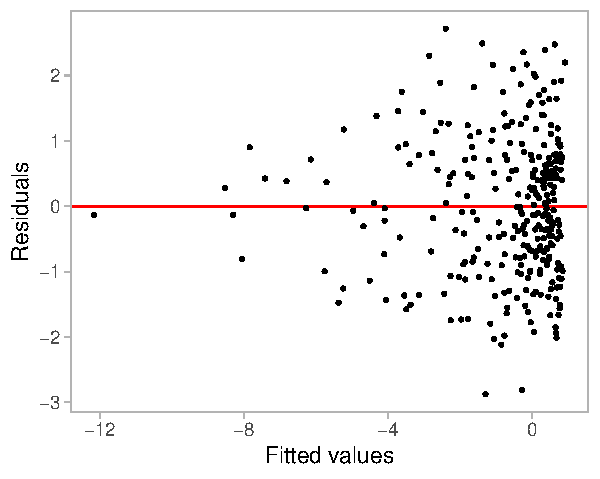
\includegraphics[width=0.5\linewidth]{paper_files/figure-latex/false-finding-1} 

}

\caption{An example residual vs fitted values plot (red line indicates 0 corresponds to the x-intercept, i.e. $y=0$). The vertical spread of the data points varies with the fitted values. This often indicates the existence of heteroskedasticity, however, here the result is due to skewed distribution of the predictors rather than heteroskedasticity. The Breusch-Pagan test rejects this residual plot at \DIFdelbeginFL \DIFdelFL{95}\DIFdelendFL \DIFaddbeginFL \DIFaddFL{5}\DIFaddendFL \% significance level ($p\text{-value} = 0.046$).}\label{fig:false-finding}
\end{figure}

The concept of visual inference, as proposed by
\citet{buja2009statistical}, provides an inferential framework \DIFdelbegin \DIFdel{to assess
}\DIFdelend \DIFaddbegin \DIFadd{for
assessing }\DIFaddend whether residual plots \DIFdelbegin \DIFdel{indeed }\DIFdelend contain visual patterns inconsistent
with the model assumptions. \DIFdelbegin \DIFdel{The fundamental idea involves testing whether the true residual plot visually differs significantly from the null plots ,
where }\DIFdelend \DIFaddbegin \DIFadd{In this framework, a }\textbf{\DIFadd{true residual
plot}} \DIFadd{refers to the residual plot obtained from the observed data under
the fitted regression model. In contrast, }\textbf{\DIFadd{null plots}} \DIFadd{are
synthetic residual plots generated under the null hypothesis \(H_0\),
where the linear regression model is correctly specified. These }\DIFaddend null
plots are \DIFdelbegin \DIFdel{plotted with residuals generated }\DIFdelend \DIFaddbegin \DIFadd{constructed by generating residuals }\DIFaddend from the residual rotation
distribution \citep{langsrud2005rotation}, which \DIFdelbegin \DIFdel{is a
distribution consistent with the null hypothesis }\DIFdelend \DIFaddbegin \DIFadd{preserves the structure
implied by }\DIFaddend \(H_0\) \DIFdelbegin \DIFdel{that the linear
regression model is correctly specified. Typically, the visual test is accomplished through }\DIFdelend \DIFaddbegin \DIFadd{(see Section \ref{sec-model-statistical-testing} for
details).
}

\DIFadd{The goal is to assess whether the true residual plot is visually
distinguishable from the null plots. This is typically done using }\DIFaddend the
lineup protocol (Figure \ref{fig:ex-lineup}), where the true residual
plot is embedded \DIFdelbegin \DIFdel{within a field of }\DIFdelend \DIFaddbegin \DIFadd{among multiple }\DIFaddend null plots. \DIFdelbegin \DIFdel{If }\DIFdelend \DIFaddbegin \DIFadd{Successful identification of
}\DIFaddend the true residual plot \DIFdelbegin \DIFdel{can be distinguished from the lineup, it
provides evidence for rejecting }\DIFdelend \DIFaddbegin \DIFadd{provides evidence against }\DIFaddend \(H_0\).

\begin{figure}[!h]

{\centering 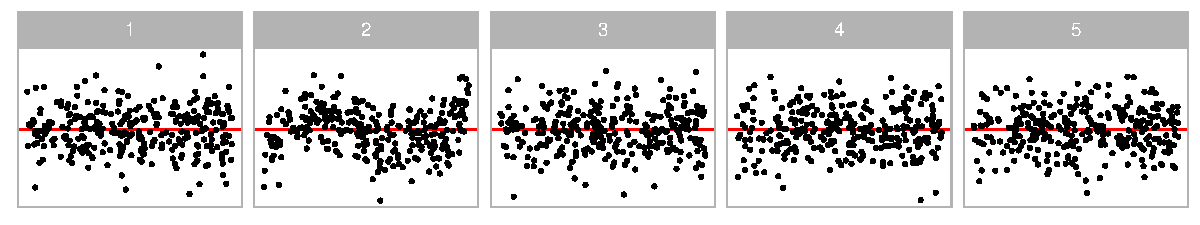
\includegraphics[width=1\linewidth]{paper_files/figure-latex/ex-lineup-1} 

}

\caption{An example lineup embedding the true residual plot among four null plots. In practice, lineups typically include 19 null plots, but a reduced set is shown here for presentation purposes. The null plots are generated via residual rotation to ensure consistency with $H_0$. Observers who have not previously seen the lineup are asked to identify the plot that appears most different. Under $H_0$ that the regression model is correctly specified, the true residual plot should be indistinguishable from the null plots, yielding a selection probability of 0.2. A small $p$-value arises when a substantial proportion of observers select the true residual plot (shown at position 2, exhibiting non-linearity).}\label{fig:ex-lineup}
\end{figure}

The practice of delivering a residual plot as a lineup is generally
regarded as a valuable approach. Beyond its application in residual
diagnostics, the lineup protocol has been integrated into the analysis
of diverse subjects. For instance, Loy and Hofmann
\citetext{\citeyear{loy2013diagnostic}; \citeyear{loy2014hlmdiag}; \citeyear{loy2015you}}
illustrated its applicability in diagnosing hierarchical linear models.
Additionally, \citet{widen2016graphical} and \citet{fieberg2024using}
demonstrated its utility in geographical and ecology research
respectively, while \citet{krishnan2021hierarchical} explored its
effectiveness in forensic examinations.

A practical limitation of the lineup protocol lies in its reliance on
human judgments \citep[see][]{li2024plot}. Unlike conventional
statistical tests that can be performed using \DIFdelbegin \DIFdel{in }\DIFdelend \DIFaddbegin \DIFadd{a }\DIFaddend statistical software,
the lineup protocol requires human evaluation of images. This
characteristic makes it less suitable for large-scale applications,
given the associated high labor costs and time requirements. There is a
substantial need to develop an approach to substitute these human
judgement\DIFdelbegin \DIFdel{with an automated reading }\DIFdelend \DIFaddbegin \DIFadd{, for example through the automated interpretation }\DIFaddend of data
plots using computer vision.

Efforts to automate plot interpretation date back to early work like
Tukey's ``Scagnostics'' \citep{tukey1985computer}, which is a set of
numerical statistics that summarize features of scatter plots.
\citet{wilkinson2005graph} expanded on this work, introducing
scagnostics based on computable measures applied to planar proximity
graphs. These measures, including, but not limited to, ``Outlying'',
``Skinny'', ``Stringy'', ``Straight'', ``Monotonic'', ``Skewed'',
``Clumpy'', and ``Striated'', aimed to characterize outliers, shape,
density, trend, coherence and other characteristics of the data.
However, such measures may not capture the full range of visual patterns
necessary for residual diagnostics \citep{buja2009statistical}. A more
promising direction lies in enabling computers to learn the relevant
visual features directly mirroring how humans intuitively interpret
plots.

Modern computer vision models rely on deep neural networks with
convolutional layers \citep{fukushima1982neocognitron}. These layers use
small, sliding windows to scan the image, performing a dot product to
extract local features and patterns. Numerous studies have demonstrated
the efficacy of convolutional layers in addressing various vision tasks,
including image recognition \citep{rawat2017deep}. Despite the
widespread use of computer vision models in fields like computer-aided
diagnosis \citep{lee2015image}, pedestrian detection
\citep{brunetti2018computer}, and facial recognition
\citep{emami2012facial}, their application in reading data plots remains
limited. While some studies have explored the use of computer vision
models for tasks such as reading recurrence plots for time series
regression \citep{ojeda2020multivariate}, time series classification
\citep{chu2019automatic, hailesilassie2019financial, hatami2018classification, zhang2020encoding},
anomaly detection \citep{chen2020convolutional}, and pairwise causality
analysis \citep{singh2017deep}, the application of reading residual
plots with computer vision models is a new field of study.

In this paper, we develop computer vision models and integrate them into
the residual plot diagnostics workflow, addressing the need for
automated visual inference. The model is a regression-based computer
vision system that takes a residual plot as input and outputs a
non-negative estimated distance \(\hat{D}\). Training and test data are
generated from a synthetic data model, simulating residual plots under
various violation scenarios, with targets defined as customized
distances \(D\) computed from the underlying data generating process,
quantifying the extent of model violations. The model \DIFdelbegin \DIFdel{performance }\DIFdelend is evaluated on
held-out test plots \DIFdelbegin \DIFdel{and compared }\DIFdelend \DIFaddbegin \DIFadd{for its ability to estimate \(\hat{D}\). In
addition, we develop a statistical testing procedure based on
\(\hat{D}\) for detecting model misspecification, and compare its
performance }\DIFaddend with classical residual diagnostic tests as well as results
from a human-subject \DIFdelbegin \DIFdel{experiment}\DIFdelend \DIFaddbegin \DIFadd{visual inference experiment using the lineup
protocol}\DIFaddend .

The paper is structured as follows. Section
\ref{sec-model-specifications} discusses \DIFdelbegin \DIFdel{various }\DIFdelend \DIFaddbegin \DIFadd{different }\DIFaddend specifications of the
computer vision models. Section
\ref{sec-model-distance-between-residual-plots} \DIFdelbegin \DIFdel{defines }\DIFdelend \DIFaddbegin \DIFadd{introduces }\DIFaddend the distance
measure used to \DIFdelbegin \DIFdel{detect }\DIFdelend \DIFaddbegin \DIFadd{quantify }\DIFaddend model violations, while Section
\ref{sec-model-distance-estimation} \DIFdelbegin \DIFdel{explains how the }\DIFdelend \DIFaddbegin \DIFadd{describes how this measure is
estimated using }\DIFaddend computer vision models\DIFdelbegin \DIFdel{estimate this distance measure}\DIFdelend \DIFaddbegin \DIFadd{, including the model
architecture, data generation, and training procedure}\DIFaddend . Section
\ref{sec-model-statistical-testing} \DIFdelbegin \DIFdel{covers the }\DIFdelend \DIFaddbegin \DIFadd{describes }\DIFaddend statistical tests based on
the estimated distance\DIFdelbegin \DIFdel{. Sections \ref{sec-model-architecture} and \ref{sec-model-data-generation} describe the model architecture and the corresponding data generation and training process, respectively. The
results are presented }\DIFdelend \DIFaddbegin \DIFadd{, and Section \ref{sec-bootstrap-assessment}
presents bootstrap-based methods for assessing the variability of
estimated distance and the stability of model misspecification
conclusions. Results are reported }\DIFaddend in Section \ref{sec-model-results}\DIFdelbegin \DIFdel{. Example
dataset applications are discussed }\DIFdelend \DIFaddbegin \DIFadd{,
followed by illustrative applications on example datasets }\DIFaddend in Section
\ref{sec-examples}. Finally, we conclude with a discussion of \DIFdelbegin \DIFdel{our findings and propose ideas
}\DIFdelend \DIFaddbegin \DIFadd{the
findings and outline directions }\DIFaddend for future research\DIFdelbegin \DIFdel{directions}\DIFdelend .

\section{Model Specifications}\label{sec-model-specifications}

There are various specifications of the computer vision model that can
be used to assess residual plots. We discuss these specifications below
focusing on the input and the output formats.

\subsection{Input Formats}\label{input-formats}

Deep learning models are sensitive to input design, and several
alternatives are available for encoding residual plots. A simple
approach involves feeding vectors of residuals and fitted values into
the model. While this format contains all relevant information, the
input length varies with sample size, which conflicts with the
fixed-shape requirements of modern vision models such as those
implemented in TensorFlow \citep{abadi2016tensorflow}. Padding can be
used to enforce uniform length but risks truncation if inputs exceed the
fixed size. Alternatively, fixed-size sampling of residual--fitted value
pairs can ensure consistency, though at the cost of some information
loss.

Another strategy is to convert residual plots into images. This enables
the use of standard convolutional architectures in computer vision such
as VGG16 \citep{simonyan2014very}. Image-based inputs offer a richer
representation by preserving the joint distribution of residuals and
fitted values in a visually interpretable format, helping models more
effectively capture spatial structure and local correlations than
vector-based formats. To ensure model generalization, it is essential to
use residual plots in a consistent style, i.e., same aesthetics, layout,
scaling and color schemes.

Using multiple residual plots as input, such as pairs, triplets, or full
lineups is also a possible option. For instance, triplet networks
\citep{chopra2005learning} can assess visual similarity if we assume
null plots are more similar to each other than to the true residual
plot, which may help distinguish null plots from true residual plots.
However, these architectures introduce complexity in training due to
weight sharing and specialized loss functions. We experimented with this
setting in a pilot study, and found multiple residual plots led to high
input resolution, high computational cost and suboptimal model
performance. Balancing accuracy, interpretability, and implementation
cost, we adopt a single residual plot in image format as the model
input.

\subsection{Output Formats}\label{output-formats}

Given the input is a single fixed-resolution image, the model output can
be defined for various tasks, including binary classification,
multiclass classification, and numeric regression.

In the binary case, the outcome may indicate whether the input image is
consistent with a null plot, as determined either by (1) the
data-generating process or (2) the outcome of a visual test based on
human judgment. The first approach models the probability that a
residual plot is not a null plot and is a viable option. In contrast,
the second relies on experimental data that are often scarce or
inconsistent across studies.

Alternatively, a multiclass outcome may classify images into categories
such as ``contains outliers'' vs.~``does not contain outliers'' or ``is
non-linear'' vs.~``not non-linear,'' among other diagnostic features.
While this approach is appealing in theory, it essentially reverts to
the traditional testing framework, where tests focus on detecting
specific types of model violations in isolation.

A third option is to produce a meaningful and interpretable numerical
measure that quantifies the strength of suspicious visual patterns
reflecting the extent of model violations, or the difficulty index for
identifying whether a residual plot has no issues. However, such
measures are often used informally in daily communications but are
rarely formalized. For supervised learning, they must be clearly defined
and reliably estimable.

In this study, we \DIFdelbegin \DIFdel{define and use a continuous distance between a true
residual plot and a theoretically ``good'' residual plot. This approach
captures the degree to which a plot deviates }\DIFdelend \DIFaddbegin \DIFadd{formulate the output as a continuous measure of
deviation }\DIFaddend from model assumptions. \DIFdelbegin \DIFdel{In
contrast, a probability output }\DIFdelend \DIFaddbegin \DIFadd{Compared to probability outputs }\DIFaddend based
on binary labels \DIFdelbegin \DIFdel{, where }\DIFdelend \DIFaddbegin \DIFadd{(}\DIFaddend true residual plots \DIFdelbegin \DIFdel{are }\DIFdelend labeled as 1 and null plots as 0\DIFdelbegin \DIFdel{, cannot express }\DIFdelend \DIFaddbegin \DIFadd{),
this formulation explicitly encodes }\DIFaddend the severity of \DIFdelbegin \DIFdel{violation. It forces }\DIFdelend \DIFaddbegin \DIFadd{violations and
avoids forcing }\DIFaddend the model to infer \DIFdelbegin \DIFdel{this information
}\DIFdelend \DIFaddbegin \DIFadd{such structure }\DIFaddend solely from the data
distribution, which \DIFdelbegin \DIFdel{may }\DIFdelend \DIFaddbegin \DIFadd{can }\DIFaddend be inefficient and discards useful prior
knowledge.

\section{Distance from a Theoretically ``Good'' Residual
Plot}\label{sec-model-distance-between-residual-plots}

\DIFdelbegin \DIFdel{To develop a computer vision model for assessing residual plots within
the visual inference framework, it is important to precisely define a
}\DIFdelend \DIFaddbegin \DIFadd{A }\DIFaddend numerical measure of ``difference'' or ``distance'' between plots \DIFdelbegin \DIFdel{. This
distance }\DIFdelend can
take the form of a basic statistical operation on pixels, such as the
sum of \DIFdelbegin \DIFdel{square differences, however, a }\DIFdelend \DIFaddbegin \DIFadd{squared differences. However, direct }\DIFaddend pixel-to-pixel \DIFdelbegin \DIFdel{comparison makes little sense in comparing residual plotswhere the main
interest would be }\DIFdelend \DIFaddbegin \DIFadd{comparisons
are not well suited to residual plots, where the primary interest lies
in }\DIFaddend structural patterns. Alternatively, \DIFdelbegin \DIFdel{it can involve
}\DIFdelend \DIFaddbegin \DIFadd{the distance can be based on
}\DIFaddend established image similarity metrics \DIFdelbegin \DIFdel{like }\DIFdelend \DIFaddbegin \DIFadd{such as }\DIFaddend the Structural Similarity
Index Measure \citep{wang2004image}, which compares images \DIFdelbegin \DIFdel{by
integrating three perception features of an image: }\DIFdelend \DIFaddbegin \DIFadd{using
}\DIFaddend contrast, luminance, and structure (related to \DIFaddbegin \DIFadd{the }\DIFaddend average, standard
deviation\DIFaddbegin \DIFadd{, }\DIFaddend and correlation of pixel values \DIFdelbegin \DIFdel{over }\DIFdelend \DIFaddbegin \DIFadd{within }\DIFaddend a window,
respectively). These \DIFdelbegin \DIFdel{image similarity
metrics are tailored for image comparison in tasks that are vastly
different }\DIFdelend \DIFaddbegin \DIFadd{metrics are designed for general image comparison
tasks that differ substantially }\DIFaddend from evaluating data plots, where only
essential plot elements \DIFdelbegin \DIFdel{require assessment \mbox{%DIFAUXCMD
\citep{chowdhury2018measuring}}\hskip0pt%DIFAUXCMD
.
A different }\DIFdelend \DIFaddbegin \DIFadd{are relevant \mbox{%DIFAUXCMD
\citep{chowdhury2018measuring}}\hskip0pt%DIFAUXCMD
.
Another }\DIFaddend direction is to define \DIFdelbegin \DIFdel{a notion of distance by integrating key plot elements
(instead of key perception features like luminance, contrast, and
structure), }\DIFdelend \DIFaddbegin \DIFadd{distance using key scatter plot
characteristics, }\DIFaddend such as those captured by scagnostics (see Section
\ref{sec-model-introduction}), \DIFdelbegin \DIFdel{but }\DIFdelend \DIFaddbegin \DIFadd{although }\DIFaddend the functional form \DIFdelbegin \DIFdel{needs to be
carefully tailored }\DIFdelend \DIFaddbegin \DIFadd{must be
carefully designed }\DIFaddend to reflect model violations meaningfully.

In this section, we introduce a distance measure between a true residual
plot and a theoretically ``good'' residual plot. This measure quantifies
the divergence between the residual distribution of a given fitted
regression model and that of a correctly specified model. \DIFdelbegin \DIFdel{The
computation }\DIFdelend \DIFaddbegin \DIFadd{Its
construction }\DIFaddend assumes knowledge of the data generating processes for \DIFaddbegin \DIFadd{both
}\DIFaddend predictors and response variables. Since these processes are often
unknown in practice, \DIFdelbegin \DIFdel{we will discuss a method to estimate this distance }\DIFdelend \DIFaddbegin \DIFadd{Section \ref{sec-model-distance-estimation}
discusses how the distance can be estimated }\DIFaddend using a computer vision
model\DIFdelbegin \DIFdel{in Section \ref{sec-model-distance-estimation}}\DIFdelend \DIFaddbegin \DIFadd{, while Section \ref{sec-model-statistical-testing} describes a
statistical test based on the estimated distance}\DIFaddend .

\subsection{Residual Distribution}\label{residual-distribution}

\DIFdelbegin \DIFdel{For a }\DIFdelend \DIFaddbegin \DIFadd{Consider the }\DIFaddend classical normal linear regression model,
\DIFdelbegin \DIFdel{\(\boldsymbol{y} = \boldsymbol{X}\boldsymbol{\beta} + \boldsymbol{e}\),
the residuals \(\hat{\boldsymbol{e}}\) are derived as the difference of
the fitted values and observed values }\DIFdelend \DIFaddbegin \DIFadd{\(\boldsymbol{y}=\boldsymbol{X}\boldsymbol{\beta}+\boldsymbol{e}\),
where }\DIFaddend \(\boldsymbol{y}\) \DIFdelbegin \DIFdel{. Suppose the
data generating process is known and the regression model is correctly
specified,
by the Frisch-Waugh-Lowell theorem \mbox{%DIFAUXCMD
\citep{frisch1933partial}}\hskip0pt%DIFAUXCMD
, residuals \(\hat{\boldsymbol{e}}\) can also be treated as random
variables and written as a
linear transformation of the error
}\DIFdelend \DIFaddbegin \DIFadd{is the \(n\times 1\) response vector,
\(\boldsymbol{X}\) is the design matrix, \(\boldsymbol{\beta}\) is a
vector of regression coefficients and }\DIFaddend \(\boldsymbol{e}\) \DIFdelbegin \DIFdel{formulated as
\(\hat{\boldsymbol{e}} = \boldsymbol{R}\boldsymbol{e}\),
where
\(\boldsymbol{R}=\boldsymbol{I}_n -\boldsymbol{X}(\boldsymbol{X}^\top\boldsymbol{X})^{-1}\boldsymbol{X}^\top\)
}\DIFdelend \DIFaddbegin \DIFadd{is the vector
of random errors. The residual vector is
\(\hat{\boldsymbol{e}}=\boldsymbol{y}-\hat{\boldsymbol{y}} = \boldsymbol{R}\boldsymbol{e}\),
where
\(\boldsymbol{R}=\boldsymbol{I}_n-\boldsymbol{X}(\boldsymbol{X}^\top\boldsymbol{X})^{-1}\boldsymbol{X}^\top\)
}\DIFaddend is the residual operator, \DIFaddbegin \DIFadd{and }\DIFaddend \(\boldsymbol{I}_n\) is \DIFdelbegin \DIFdel{a \(n\) by \(n\)
identity matrix, and \(n\) is the number of observations}\DIFdelend \DIFaddbegin \DIFadd{the \(n\times n\)
identity matrix}\DIFaddend .

\DIFdelbegin \DIFdel{One of the assumptions of the classical normal linear regression model
is that the error }\DIFdelend \DIFaddbegin \DIFadd{Under the classical assumptions
\(\boldsymbol{e}\sim \mathcal{N}(\boldsymbol{0}_n,\sigma^2\boldsymbol{I}_n)\),
the residuals are also Gaussian, since they are a linear transformation
of }\DIFaddend \(\boldsymbol{e}\)\DIFdelbegin \DIFdel{follows a multivariate normal
distribution with zero mean and constant variance, i.e.,
\(\boldsymbol{e} \sim N(\boldsymbol{0}_n,\sigma^2\boldsymbol{I}_n)\). It
follows that the distribution of residuals \(\hat{\boldsymbol{e}}\) can
be characterized by a certain probability distribution, denoted as \(Q\), which is transformed from the
multivariate normal distribution.
This }\DIFdelend \DIFaddbegin \DIFadd{. We refer to this induced distribution as the
}\DIFaddend reference distribution \(Q\)\DIFdelbegin \DIFdel{summarizes what ``good'' residuals
should follow given the design matrix }\DIFdelend \DIFaddbegin \DIFadd{, which characterizes the residual behaviour
under correct model specification and depends only on
}\DIFaddend \(\boldsymbol{X}\)\DIFdelbegin \DIFdel{is known and fixed}\DIFdelend .

\DIFdelbegin \DIFdel{Suppose the design matrix }\DIFdelend \DIFaddbegin \DIFadd{If }\DIFaddend \(\boldsymbol{X}\) has \DIFdelbegin \DIFdel{linearly independent
columns, the trace of the hat matrix
\(\boldsymbol{H} = \boldsymbol{X}(\boldsymbol{X}^\top\boldsymbol{X})^{-1}\boldsymbol{X}^\top\)
equals the number of columns in \(\boldsymbol{X}\) denoted as }\DIFdelend \DIFaddbegin \DIFadd{full column rank }\DIFaddend \(k\)\DIFdelbegin \DIFdel{. As
a result, the rank of \(\boldsymbol{R}\) is \(n - k\), and
}\DIFdelend \DIFaddbegin \DIFadd{, then
\(\text{rank}(\boldsymbol{R}) = n - k\), and
\(\mathrm{cov}(\hat{\boldsymbol{e}})=\sigma^2\boldsymbol{R}\) is
singular. Hence, }\DIFaddend \(Q\) is a degenerate \DIFdelbegin \DIFdel{multivariate distribution. To capture the characteristics of
\(Q\), such as moments, we can simulate a large number of
\(\boldsymbol{\varepsilon}\) and transform it to \(\boldsymbol{e}\) to
get the empirical estimates. For the purpose of this study, we replaced
the variance-covariance matrix of residuals
\(\text{cov}(\boldsymbol{e}, \boldsymbol{e}) = \boldsymbol{R}\sigma^2\boldsymbol{R}^\top = \boldsymbol{R}\sigma^2\)
with a full-rank diagonal matrix
\(\text{diag}(\boldsymbol{R}\sigma^2)\), where \(\text{diag}(.)\) sets
the non-diagonal entries of a matrix to zeros. The resulting
distribution for \(Q\) was
\(N(\boldsymbol{0}_n, \text{diag}(\boldsymbol{R}\sigma^2))\). This
replacement ensures a }\DIFdelend \DIFaddbegin \DIFadd{Gaussian supported on an
\((n-k)\)-dimensional subspace. To obtain a }\DIFaddend non-degenerate \DIFdelbegin \DIFdel{distribution, which is required for computing the distance defined }\DIFdelend \DIFaddbegin \DIFadd{reference
distribution required for the distance computation }\DIFaddend in Section
\ref{sec-distance-of-p-from-q}\DIFaddbegin \DIFadd{, we replace \(\sigma^2\boldsymbol{R}\)
with its diagonal approximation,
\(\mathrm{diag}(\sigma^2\boldsymbol{R})\), yielding
\(Q \approx \mathcal{N}\left(\boldsymbol{0}_n,\mathrm{diag}(\sigma^2\boldsymbol{R})\right)\)}\DIFaddend .

\DIFdelbegin \DIFdel{Distribution }\DIFdelend \DIFaddbegin \DIFadd{The reference distribution }\DIFaddend \(Q\) \DIFdelbegin \DIFdel{is derived from the correctly specified model
.
However, if the model is misspecified, then the actual distribution of
residuals denoted as }\DIFdelend \DIFaddbegin \DIFadd{corresponds to the correct model
specification. Under misspecification, the residuals follow a different
distribution }\DIFaddend \(P\)\DIFdelbegin \DIFdel{, will be different
from \(Q\)}\DIFdelend . For example, \DIFdelbegin \DIFdel{if the data generating process contains }\DIFdelend \DIFaddbegin \DIFadd{omitted }\DIFaddend variables correlated with
\DIFdelbegin \DIFdel{any
column of }\DIFdelend \(\boldsymbol{X}\) \DIFdelbegin \DIFdel{but are missing from \(\boldsymbol{X}\), causing an omitted variable problem, }\DIFdelend \DIFaddbegin \DIFadd{alter the residual structure, causing }\DIFaddend \(P\) \DIFdelbegin \DIFdel{will be different }\DIFdelend \DIFaddbegin \DIFadd{to
deviate }\DIFaddend from \(Q\)\DIFdelbegin \DIFdel{because the residual operator obtained from the fitted regression model
will not be the same as \(\boldsymbol{R}\). Besides, if the
\(\boldsymbol{\varepsilon}\) follows a non-normal distribution such as a
multivariate lognormaldistribution, \(P\) will usually be skewed and has a long tail}\DIFdelend . \DIFaddbegin \DIFadd{Similarly, non-Gaussian error distributions
(e.g.~multivariate lognormal) induce skewness and heavier tails.
}\DIFaddend 

\subsection{\texorpdfstring{Distance of \(P\) from
\(Q\)}{Distance of P from Q}}\label{sec-distance-of-p-from-q}

\DIFdelbegin \DIFdel{Defining a proper distance between distributions is usually easier than
defining a proper distance between data plots. Given }\DIFdelend \DIFaddbegin \DIFadd{We define the distance of }\DIFaddend the true residual distribution \(P\) \DIFdelbegin \DIFdel{and }\DIFdelend \DIFaddbegin \DIFadd{from }\DIFaddend the
reference residual distribution \(Q\) \DIFdelbegin \DIFdel{, we
used a distance measure based on Kullback-Leibler divergence \mbox{%DIFAUXCMD
\citep{kullback1951information}}\hskip0pt%DIFAUXCMD
to quantify the difference between two
distributions as
}%DIFDELCMD < 

%DIFDELCMD < %%%
\DIFdelend \DIFaddbegin \DIFadd{based on the Kullback--Leibler
divergence \mbox{%DIFAUXCMD
\citep{kullback1951information}}\hskip0pt%DIFAUXCMD
:
}\DIFaddend \begin{equation} \label{eq:kl-0}
D = \log\left(1 + D_{KL}(P \| Q)\right),
\end{equation} \DIFdelbegin %DIFDELCMD < 

%DIFDELCMD < %%%
\DIFdelend \DIFaddbegin \noindent \DIFaddend where \(D_{KL}(P \| Q)\) is defined as
\DIFdelbegin %DIFDELCMD < 

%DIFDELCMD < %%%
\DIFdelend \begin{equation} \label{eq:kl-1}
D_{KL}(P \| Q) = \int_{\mathbb{R}^{n}}\log\DIFdelbegin \DIFdel{\frac{p(\boldsymbol{e})}{q(\boldsymbol{e})}}\DIFdelend \DIFaddbegin \DIFadd{\frac{p(\hat{\boldsymbol{e}})}{q(\hat{\boldsymbol{e}})}}\DIFaddend p(\DIFdelbegin %DIFDELCMD < \boldsymbol{e}%%%
\DIFdelend \DIFaddbegin \hat{\boldsymbol{e}}\DIFaddend )d\DIFdelbegin %DIFDELCMD < \boldsymbol{e}%%%
\DIFdelend \DIFaddbegin \hat{\boldsymbol{e}}\DIFaddend ,
\end{equation} \DIFdelbegin %DIFDELCMD < 

%DIFDELCMD < %%%
\DIFdelend \noindent and \DIFdelbegin \DIFdel{\(p(.)\) and \(q(.)\) }\DIFdelend \DIFaddbegin \DIFadd{\(p(\cdot)\) and \(q(\cdot)\) }\DIFaddend are the
probability density functions for \DIFdelbegin \DIFdel{distribution }\DIFdelend \(P\) and \DIFdelbegin \DIFdel{distribution }\DIFdelend \(Q\), respectively.

This \DIFdelbegin \DIFdel{distance measure was first proposed in \mbox{%DIFAUXCMD
\citet{li2024plot} }\hskip0pt%DIFAUXCMD
, which
was mainly designed for measuring }\DIFdelend \DIFaddbegin \DIFadd{measure was introduced in \mbox{%DIFAUXCMD
\citet{li2024plot} }\hskip0pt%DIFAUXCMD
to quantify }\DIFaddend the effect
size of non-linearity and heteroskedasticity in \DIFdelbegin \DIFdel{a residual plot. \mbox{%DIFAUXCMD
\citet{li2024plot} }\hskip0pt%DIFAUXCMD
has derived
that, for a classical normal linear regression model that omits
necessary higher-order predictors \(\boldsymbol{Z}\) and the corresponding parameter \(\boldsymbol{\beta}_z\),
while incorrectly
assuming
\(\boldsymbol{\varepsilon} \sim N(\boldsymbol{0}_n,\sigma^2\boldsymbol{I}_n)\),
but in fact
\(\boldsymbol{\varepsilon} \sim N(\boldsymbol{0}_n, \boldsymbol{V})\)
where }\DIFdelend \DIFaddbegin \DIFadd{residual plots. In the
presence of model misspecification, if the error structure deviates from
\(\boldsymbol{e} \sim \mathcal{N}(\boldsymbol{0}_n,\sigma^2\boldsymbol{I}_n)\),
for instance with covariance }\DIFaddend \(\boldsymbol{V}\) \DIFdelbegin \DIFdel{is an arbitrary symmetric positive
semi-definite matrix, \(P\) can be represented as
\(N(\boldsymbol{R}\boldsymbol{Z}\boldsymbol{\beta}_z, \text{diag}(\boldsymbol{R}\boldsymbol{V}\boldsymbol{R}))\).
Note that the variance-covariance matrix was replaced with the diagonal matrix to ensure it is
a full-rank matrix}\DIFdelend \DIFaddbegin \DIFadd{and omitted higher-order
terms \(\boldsymbol{Z}\boldsymbol{\beta}_z\) correlated with
\(\boldsymbol{X}\), the induced residual distribution can be expressed
as
\(P = \mathcal{N}(\boldsymbol{R}\boldsymbol{Z}\boldsymbol{\beta}_z, \text{diag}(\boldsymbol{R}\boldsymbol{V}\boldsymbol{R}))\),
where the diagonal approximation ensures non-degenerate covariance
matrix. The transformation \(D = \log(1 + D_{KL})\) compresses large
values of \(D_{KL}\), improves numerical stability during estimation
(Section \ref{sec-model-distance-estimation}), and ensures that \(D\) is
well-defined when \(D_{KL} = 0\)}\DIFaddend .

Since \DIFdelbegin \DIFdel{both }\DIFdelend \(P\) and \(Q\) are \DIFdelbegin \DIFdel{adjusted to be multivariate normal
distributions, Equation \ref{eq:kl-1} can be further expanded to
}%DIFDELCMD < 

%DIFDELCMD < %%%
\DIFdelend \DIFaddbegin \DIFadd{taken as non-degenerate Gaussian
distributions, the KL divergence admits the closed form
}\DIFaddend \begin{equation} \label{eq:kl-2}
D_{KL}(P \| Q) = \frac{1}{2}\left(\log\frac{|\boldsymbol{W}|}{|\text{diag}(\boldsymbol{R}\sigma^2)|} - n + \text{tr}(\boldsymbol{W}^{-1}\text{diag}(\boldsymbol{R}\sigma^2)) + \boldsymbol{\mu}_z^\top\boldsymbol{W}^{-1}\boldsymbol{\mu}_z\right),
\end{equation} \DIFdelbegin %DIFDELCMD < 

%DIFDELCMD < %%%
\DIFdelend \noindent where
\(\boldsymbol{\mu}_z = \boldsymbol{R}\boldsymbol{Z}\boldsymbol{\beta}_z\),
and
\(\boldsymbol{W} = \text{diag}(\boldsymbol{R}\boldsymbol{V}\boldsymbol{R})\).
The assumed error variance \(\sigma^2\) is set to be
\(\text{tr}(\boldsymbol{V})/n\), which is the expectation of the
estimated variance.

\subsection{\texorpdfstring{Non-normal
\(P\)}{Non-normal P}}\label{non-normal-p}

\DIFdelbegin \DIFdel{For non-normal error \(\boldsymbol{\varepsilon}\), the true }\DIFdelend \DIFaddbegin \DIFadd{When the error vector \(\boldsymbol{e}\) is non-Gaussian, the induced
}\DIFaddend residual distribution \(P\) is \DIFdelbegin \DIFdel{unlikely to be a multivariate normal distribution. Thus, Equation \ref{eq:kl-2} given in \mbox{%DIFAUXCMD
\citet{li2024plot} }\hskip0pt%DIFAUXCMD
will not be
applicableto models violating the normality assumption.
}%DIFDELCMD < 

%DIFDELCMD < %%%
\DIFdel{To evaluate the Kullback-Leibler divergence of non-normal \(P\) from \(Q\), the fallback is to evaluate Equation
\ref{eq:kl-1}numerically. However, since \(\boldsymbol{e}\) is a linear transformation of
non-normal random variables, it is very common that the general form of
\(P\) is unknown, meaning that we can not easily compute
\(p(\boldsymbol{e})\) using a well-known probability density function.
Additionally, even if \(p(\boldsymbol{e})\) can be calculated for any
\(\boldsymbol{e} \in \mathbb{R}^n\), it will be very difficult to do
numerical }\DIFdelend \DIFaddbegin \DIFadd{generally non-Gaussian and typically
unavailable in closed form. Consequently, the Gaussian closed-form
expression in Equation \ref{eq:kl-2} is no longer applicable, and the KL
divergence must instead be evaluated from its definition in Equation
\ref{eq:kl-1}. This requires high-dimensional }\DIFaddend integration over the
\DIFaddbegin \DIFadd{residual space, rendering direct evaluation impractical for large }\DIFaddend \(n\)\DIFdelbegin \DIFdel{-dimensional space, because \(n\)
could be potentially very large }\DIFdelend .

\DIFdelbegin \DIFdel{In order to approximate \(D_{KL}(P \| Q)\) in a practically computable
manner, the elements of \(\boldsymbol{e}\) are assumed to be independentof each other}\DIFdelend \DIFaddbegin \DIFadd{To obtain a tractable approximation, we assume that the residual
components \(\{\hat{e}_i\}_{i=1}^n\) are mutually independent, so that
\(p(\hat{\boldsymbol{e}}) \approx \prod_{i=1}^n p_i(\hat{e}_i)\) and
\(q(\hat{\boldsymbol{e}}) \approx \prod_{i=1}^n q_i(\hat{e}_i)\)}\DIFaddend . This
assumption \DIFdelbegin \DIFdel{solves both of the issues mentioned
above. First, we no longer need to integrate over \(n\) random
variables. The result of Equation \ref{eq:kl-1} is now the sum of the
Kullback-Leibler divergence evaluated for
each individual residual due
to the assumption of independence between observations. Second,
it is
not required to know the joint probability density \(p(\boldsymbol{e})\)
any more. Instead, the evaluation of Kullback-Leibler divergence for an
individual residual relies on the knowledge of the marginal density
\(p_i(e_i)\), where \(e_i\) is the \(i\)-th residual for
\(i = 1, ..., n\). This is much easier to approximate through
simulation. It is also worth mentioning that this independence
assumption generally will not hold if \(\text{cov}(e_i, e_j) \neq 0\)
for any \(1 \leq i < j \leq n\), but its existence is essential for reducing the }\DIFdelend \DIFaddbegin \DIFadd{holds for
\(Q \approx \mathcal{N}\left(\boldsymbol{0}_n,\mathrm{diag}(\sigma^2\boldsymbol{R})\right)\),
which has independent components, but generally does not hold for \(P\).
Nevertheless, it removes the need for high-dimensional integration and
reduces the computation to univariate densities, substantially lowering
}\DIFaddend computational cost.

\DIFdelbegin \DIFdel{Given \(\boldsymbol{X}\) }\DIFdelend \DIFaddbegin \DIFadd{Under this factorisation, the KL divergence decomposes additively:
}\[\DIFadd{D_{KL}(P \| Q) \approx \sum_{i=1}^n \int_{\mathbb{R}} p_i(\hat{e}_i)\log\frac{p_i(\hat{e}_i)}{q_i(\hat{e}_i)} d\hat{e}_i = \sum_{i=1}^n \mathbb{E}_{p_i}\left[\log\frac{p_i(\hat{e}_i)}{q_i(\hat{e}_i)}\right],}\]
\noindent \DIFadd{where \(p_i\) }\DIFaddend and \DIFdelbegin \DIFdel{\(\boldsymbol{\beta}\), the algorithm for
approximating Equation \ref{eq:kl-1} starts from simulating \(m\) sets
of observed values \(\boldsymbol{y}\) according to the data generating
process. The observed values are stored in a matrix \(\boldsymbol{A}\)
with \(n\) rows and \(m\) columns, where each column of
\(\boldsymbol{A}\) is a set of observed values.
Then,
we can get \(m\)
sets of realized values of \(\boldsymbol{e}\) stored in the matrix
\(\boldsymbol{B}\) by applying the residual operator
\(\boldsymbol{B} = \boldsymbol{R}\boldsymbol{A}\). Furthermore, kernel
density estimation (KDE) with Gaussian kernel and optimal }\DIFdelend \DIFaddbegin \DIFadd{\(q_i\) denote the marginal densities of
\(\hat{e}_i\) under \(P\) and \(Q\), respectively.
}

\DIFadd{We approximate the expectation via Monte Carlo simulation. Specifically,
we generate independent samples \(\{\boldsymbol{e}^{(j)}\}_{j=1}^m\)
from the error distribution and obtain residual vectors
\(\boldsymbol{B}_j = \boldsymbol{R}\boldsymbol{e}^{(j)}\). The marginal
density \(p_i\) is then estimated from \(\{B_{ij}\}_{j=1}^m\) using a
Gaussian kernel density estimator with }\DIFaddend bandwidth selected by \DIFdelbegin \DIFdel{the }\DIFdelend Silverman's
rule of thumb \citep{silverman2018density}\DIFdelbegin \DIFdel{is applied on each row of \(\boldsymbol{B}\) to estimate \(p_i(e_i)\)
for \(i = 1, ..., n\). The KDE computation can be done by the
}\texttt{\DIFdel{density}} %DIFAUXCMD
\DIFdel{function in R.
}%DIFDELCMD < 

%DIFDELCMD < %%%
\DIFdel{Since the Kullback-Leibler divergence can be viewed as the expectation
of the log-likelihood ratio between distribution \(P\) and distribution
\(Q\) evaluated on distribution \(P\), we can reuse the simulated
residuals in matrix \(\boldsymbol{B}\) to estimate the expectation by
the sample mean. With the independence assumption, for non-normal \(P\)}\DIFdelend , \DIFdelbegin \DIFdel{\(D_{KL}(P \| Q)\) can be approximated by
}%DIFDELCMD < 

%DIFDELCMD < %%%
\begin{align*} \DIFdel{%DIFDELCMD < \label{eq:kl-3}%%%
D_{KL}(P \| Q) }&\DIFdel{\approx \sum_{i = 1}^{n} \hat{D}_{KL}^{(i)}(P \| Q), \quad
\hat{D}_{KL}^{(i)}(P \| Q) = \frac{1}{m}\sum_{j = 1}^{m} \log\frac{\hat{p}_i(B_{ij})}{q(B_{ij})},
}\end{align*}%DIFAUXCMD
%DIFDELCMD < 

%DIFDELCMD < \noindent %%%
\DIFdel{where \(\hat{D}_{KL}^{(i)}(P \| Q)\) is the estimator of the
Kullback-Leibler divergence for an individual residual \(e_i\),
}\DIFdelend \DIFaddbegin \DIFadd{where }\DIFaddend \(B_{ij}\) \DIFdelbegin \DIFdel{is }\DIFdelend \DIFaddbegin \DIFadd{denotes }\DIFaddend the
\(i\)-th \DIFdelbegin \DIFdel{row and \(j\)-th column entry of the matrix
\(\boldsymbol{B}\), \(\hat{p}_i(.)\) is the kernel density
estimator of
\(p_i(.)\), \(q(.)\) is the normal density function with mean zero and
an assumed variance estimated as
\(\hat{\sigma}^2 = \sum_{b \in vec(\boldsymbol{B})}(b - \sum_{b \in vec(\boldsymbol{B})} b/nm)^2/(nm - 1)\), and \(vec(.)\) is the vectorization operator which turns a
\(n \times m\) matrix into a \(nm \times 1\) column vector by stacking
the columns of the matrix on top of each other}\DIFdelend \DIFaddbegin \DIFadd{component of \(\boldsymbol{B}_j\). This yields
}\[\DIFadd{D_{KL}(P \| Q) \approx \sum_{i=1}^n \mathbb{E}_{p_i}\left[\log\frac{p_i(\hat{e}_i)}{q_i(\hat{e}_i)}\right] \approx \sum_{i=1}^n\frac{1}{m}\sum_{j=1}^m \log\frac{\hat{p}_i(B_{ij})}{q_i(B_{ij})},}\]
\noindent \DIFadd{where \(q_i(\cdot)\) denotes the Gaussian reference density
with variance \(\hat{\sigma}^2R_{ii}\), with
\(\hat{\sigma}^2 = \frac{1}{nm - 1}\sum_{b \in \mathrm{vec}(\boldsymbol{B})} \left(b - \bar{b}\right)^2\)
and
\(\bar{b} = \frac{1}{nm}\sum_{b \in \mathrm{vec}(\boldsymbol{B})} b\)}\DIFaddend .

\section{Distance Estimation \DIFaddbegin \DIFadd{Using Computer Vision
Models}\DIFaddend }\label{sec-model-distance-estimation}

\DIFdelbegin \DIFdel{We previously defined a distance measure (Equation \ref{eq:kl-0} ) to
quantify }\DIFdelend \DIFaddbegin \DIFadd{The distance measure defined in Equation \ref{eq:kl-0} quantifies }\DIFaddend the
difference between the true residual distribution \(P\) and \DIFdelbegin \DIFdel{an ideal }\DIFdelend \DIFaddbegin \DIFadd{the
}\DIFaddend reference distribution \(Q\). However, \DIFdelbegin \DIFdel{this distance measure
}\DIFdelend \DIFaddbegin \DIFadd{it }\DIFaddend can only be computed when the
\DIFdelbegin \DIFdel{data generating }\DIFdelend \DIFaddbegin \DIFadd{data-generating }\DIFaddend process is known\DIFdelbegin \DIFdel{. In
reality, we often have no knowledge about the data generating process,
otherwise we do not need to do a residual diagnostic in the first place}\DIFdelend \DIFaddbegin \DIFadd{, which is rarely the case in practice}\DIFaddend .

To estimate this distance from a residual plot, we \DIFdelbegin \DIFdel{proposed }\DIFdelend \DIFaddbegin \DIFadd{define }\DIFaddend a computer
vision estimator \DIFdelbegin \DIFdel{\(\hat{D}\) formulated as
}%DIFDELCMD < 

%DIFDELCMD < %%%
\DIFdelend \begin{equation*} \label{eq:d-approx}
\hat{D} = f_{CV}(V_{h \times w}(\boldsymbol{e}, \hat{\boldsymbol{y}})\DIFaddbegin \DIFadd{, }\boldsymbol{s}\DIFaddend ),
\end{equation*} \DIFdelbegin %DIFDELCMD < 

%DIFDELCMD < %%%
\DIFdelend \noindent where \DIFdelbegin \DIFdel{\(V_{h \times w}(.)\) renders the
}\DIFdelend \DIFaddbegin \DIFadd{\(V_{h \times w}(\cdot)\) denotes the
rendering function that coverts a }\DIFaddend residuals vs.~fitted values plot \DIFdelbegin \DIFdel{as }\DIFdelend \DIFaddbegin \DIFadd{into
}\DIFaddend an \(h \times w\) RGB image, \DIFdelbegin \DIFdel{and \(f_{CV}(.)\) }\DIFdelend \DIFaddbegin \DIFadd{with h and w denoting the image height and
width (in pixels), respectively. Here, \(\boldsymbol{s}\) is a vector of
auxiliary features including scagnostics measures and sample size, and
\(f_{CV}(\cdot)\) }\DIFaddend maps the image \DIFaddbegin \DIFadd{and auxiliary features }\DIFaddend to an estimated
distance \(\hat{D} \in [0, +\infty)\). Details of the model architecture
\DIFaddbegin \DIFadd{and training procedure }\DIFaddend are provided in \DIFdelbegin \DIFdel{Section
\ref{sec-model-architecture} , and the training procedure is described in Section \ref{sec-model-data-generation}. }\DIFdelend \DIFaddbegin \DIFadd{Sections
\ref{sec-model-architecture} and \ref{sec-model-data-generation},
respectively.
}\DIFaddend 

\DIFaddbegin \DIFadd{The auxiliary feature vector \(\boldsymbol{s}\) is included to
complement information encoded in the residual plot image. While
\(V_{h \times w}(\cdot)\) captures visual patterns of misspecification,
certain attributes such as sample size are not recoverable from the
image. In addition, we include scagnostics as useful graph-based
summaries of scatter plot structure, which have been shown to be
effective descriptors of shape, clustering, and outliers in exploratory
data analysis.
}

\DIFaddend The distance estimator \(\hat{D}\) \DIFdelbegin \DIFdel{allows us to assess }\DIFdelend \DIFaddbegin \DIFadd{quantifies }\DIFaddend how closely the residuals
resemble \DIFdelbegin \DIFdel{an ideal distribution and use }\DIFdelend \DIFaddbegin \DIFadd{the reference distribution \(Q\) and, after adjusting for
sample size effects, can be used }\DIFaddend as an index of model violation severity
(see Appendix D for details). However, \DIFaddbegin \DIFadd{since a single residual plot may
not fully characterize the underlying residual distribution, }\DIFaddend \(\hat{D}\)
is not expected to equal the true distance \(D\)\DIFdelbegin \DIFdel{, as a single residual plot
may not capture all characteristics of the residual distribution. For
}\DIFdelend \DIFaddbegin \DIFadd{. Residual plots
generated from }\DIFaddend the same distribution \(P\) \DIFdelbegin \DIFdel{, simulated plots can }\DIFdelend \DIFaddbegin \DIFadd{may also }\DIFaddend vary visually,
\DIFdelbegin \DIFdel{especially with }\DIFdelend \DIFaddbegin \DIFadd{particularly for }\DIFaddend small \(n\), \DIFdelbegin \DIFdel{leading to }\DIFdelend \DIFaddbegin \DIFadd{introducing }\DIFaddend estimation error that depends
on \DIFdelbegin \DIFdel{how representative the input plot is.
}\DIFdelend \DIFaddbegin \DIFadd{the representativeness of the input plot.
}\DIFaddend 

\DIFdelbegin \section{\DIFdel{Statistical Testing}}%DIFAUXCMD
\addtocounter{section}{-1}%DIFAUXCMD
%DIFDELCMD < \label{sec-model-statistical-testing}
%DIFDELCMD < 

%DIFDELCMD < %%%
\subsection{\DIFdel{Lineup Evaluation}}%DIFAUXCMD
\addtocounter{subsection}{-1}%DIFAUXCMD
%DIFDELCMD < \label{sec-model-lineup-evaluation}
%DIFDELCMD < 

%DIFDELCMD < %%%
\DIFdel{Theoretically, the distance \(D\) for a correctly specified model is
\(0\), as \(P = Q\). However, a computer vision model may not predict
\(\hat{D} = 0\) for a null plot. For example, Figure
\ref{fig:false-finding} shows a null plot with a pattern suggestive of heteroskedasticity. The model can not discern whether such patterns
arise from heteroskedasticity or from skewed fitted values.
Additionally, some null plots could have outliers or strong visual
patterns due to randomness, and a reasonable model will try to summarize
those information into the prediction, resulting in \(\hat{D} > 0\).
This is not problematic when \(\hat{D}\) is large, as strong visual
signals typically justify rejection of \(H_0\). But when \(\hat{D}\) is
moderate, it is insufficient alone for decision-making.
}%DIFDELCMD < 

%DIFDELCMD < %%%
\DIFdel{To address this issue we can adhere to the paradigm of visual inference,
by comparing the estimated distance \(\hat{D}\) to the estimated
distances for the null plots in a lineup. Specifically, if a lineup
comprises 20 plots, \(H_0\) will be rejected if \(\hat{D}\) exceeds the
maximum estimated distance among the 19 null plots, denoted as
\(\max\limits_{1 \leq i \leq 19} {\hat{D}_{null}^{(i)}}\), where
\(\hat{D}_{null}^{(i)}\) represents the estimated distance for the
\(i\)-th null plot.
This approach is conceptually equivalent to the
typical lineup protocol requiring a 95\% significance level, where
\(H_0\) is rejected if the data plot is identified as the most distinct
plot by the sole observer.
}%DIFDELCMD < 

%DIFDELCMD < %%%
\DIFdel{Moreover, if the number of plots in a lineup, denoted by \(m\), is
sufficiently large, the empirical distribution of
\(\hat{D}_{null}^{(i)}\) can be viewed as an approximation to the null
distribution of the estimated distance. Consequently, quantiles of the
null distribution can be estimated using the sample quantiles and used
for decision-making purposes. This follows the standard simulation-based
approach for approximating the sampling distribution of a test statistic
in traditional statistics. Details of the computation of sample
quantiles can be found in \mbox{%DIFAUXCMD
\citet{hyndman1996sample}}\hskip0pt%DIFAUXCMD
. For instance, if
\(\hat{D}\) is greater than or equal to the 95\% sample quantile,
denoted as \(Q_{null}(0.95)\), we can conclude that the estimated
distance for the true residual plot is significantly different from the
estimated distance for null plots at the 95\% significance level. In
practice, at least 100 null plots are typically required for stable
estimate of the null distribution, though more may be necessary if the
distribution exhibits heavy tails. Alternatively, a \(p\)-value can be
defined as the probability, under \(H_0\), of observing a distance at
least as large as \(\hat{D}\), and it can be estimated as
\(\frac{1}{m} + \frac{1}{m}\sum_{i=1}^{m-1}I\left(\hat{D}_{null}^{(i)} \geq \hat{D}\right)\).
}%DIFDELCMD < 

%DIFDELCMD < %%%
\DIFdel{To reduce computational cost, a pre-computed lattice of \(\hat{D}\)
quantiles under \(H_0\) for various sample sizes can be used. By
matching observed values to the closest entries in this lattice,
approximate \(p\)-values can be obtained efficiently, with minor loss of
precision.
}%DIFDELCMD < 

%DIFDELCMD < %%%
\DIFdelend \subsection{\DIFdelbegin \DIFdel{Bootstrapping}\DIFdelend \DIFaddbegin \DIFadd{Model Architecture}\DIFaddend }\DIFdelbegin %DIFDELCMD < \label{bootstrapping}
%DIFDELCMD < 

%DIFDELCMD < %%%
\DIFdel{Bootstrap methods are commonly used in linear regression to estimate
parameter variability without strong distributional assumptions
\mbox{%DIFAUXCMD
\citep{davison1997bootstrap, efron1994introduction}}\hskip0pt%DIFAUXCMD
. This involves
resampling observations with replacement and refitting the model.
}%DIFDELCMD < 

%DIFDELCMD < %%%
\DIFdel{Similarly, we can apply bootstrapping to the estimated distance
\(\hat{D}\). For each bootstrap sample \(i = 1, \dots, n_{boot}\), we
obtain a refitted model \(M^{(i)}_{boot}\), a corresponding residual
plot \(V^{(i)}_{boot}\), and a predicted distance
\(\hat{D}^{(i)}_{boot}\). If we are interested in the variation of
\(\hat{D}\), the distribution of \(\hat{D}^{(i)}_{boot}\) can be used to
construct confidence intervals.
}%DIFDELCMD < 

%DIFDELCMD < %%%
\DIFdel{Alternatively, since each \(M_{boot}^{(i)}\) has its own residual
distribution, a new approximated null distribution can be construed and
the corresponding 95\% sample quantile \(Q_{boot}^{(i)}(0.95)\) can be
computed. Then, if \(\hat{D}_{boot}^{(i)} \geq Q_{boot}^{(i)}(0.95)\),
\(H_0\) will be rejected for \(M_{boot}^{(i)}\). The ratio of rejected
\(M_{boot}^{(i)}\) among all the refitted models reflects how often the
assumed regression model are considered to be misspecified if data were
repeatedly drawn from the same process. But this approach is
computationally very expensive because it requires
\(n_{boot} \times (n_{null} + 1)\) times of residual plot assessment. In
practice, \(Q_{null}(0.95)\) can be used to replace
\(Q_{boot}^{(i)}(0.95)\) in the computation.
}%DIFDELCMD < 

%DIFDELCMD < %%%
\section{\DIFdel{Model Architecture}}%DIFAUXCMD
\addtocounter{section}{-1}%DIFAUXCMD
\DIFdelend \label{sec-model-architecture}

The architecture of the computer vision model \(f_{CV}\) is adapted from
the well-established VGG16 architecture \citep{simonyan2014very}. While
more recent architectures like ResNet \citep{he2016deep} and
DenseNet\citep{huang2017densely}, have achieved even greater
performance, VGG16 remains a solid choice for many applications due to
its simplicity and effectiveness. Our decision to use VGG16 aligns with
our goal of starting with a proven and straightforward model. Figure
\ref{fig:cnn-diag} \DIFdelbegin \DIFdel{provides a diagram of the architecture. More details
about the neural network layers used in this study are provided in the
Appendix B
}\DIFdelend \DIFaddbegin \DIFadd{illustrates the architecture, while Appendix B
provides detailed layer specifications}\DIFaddend .

\begin{figure}[!h]

{\centering 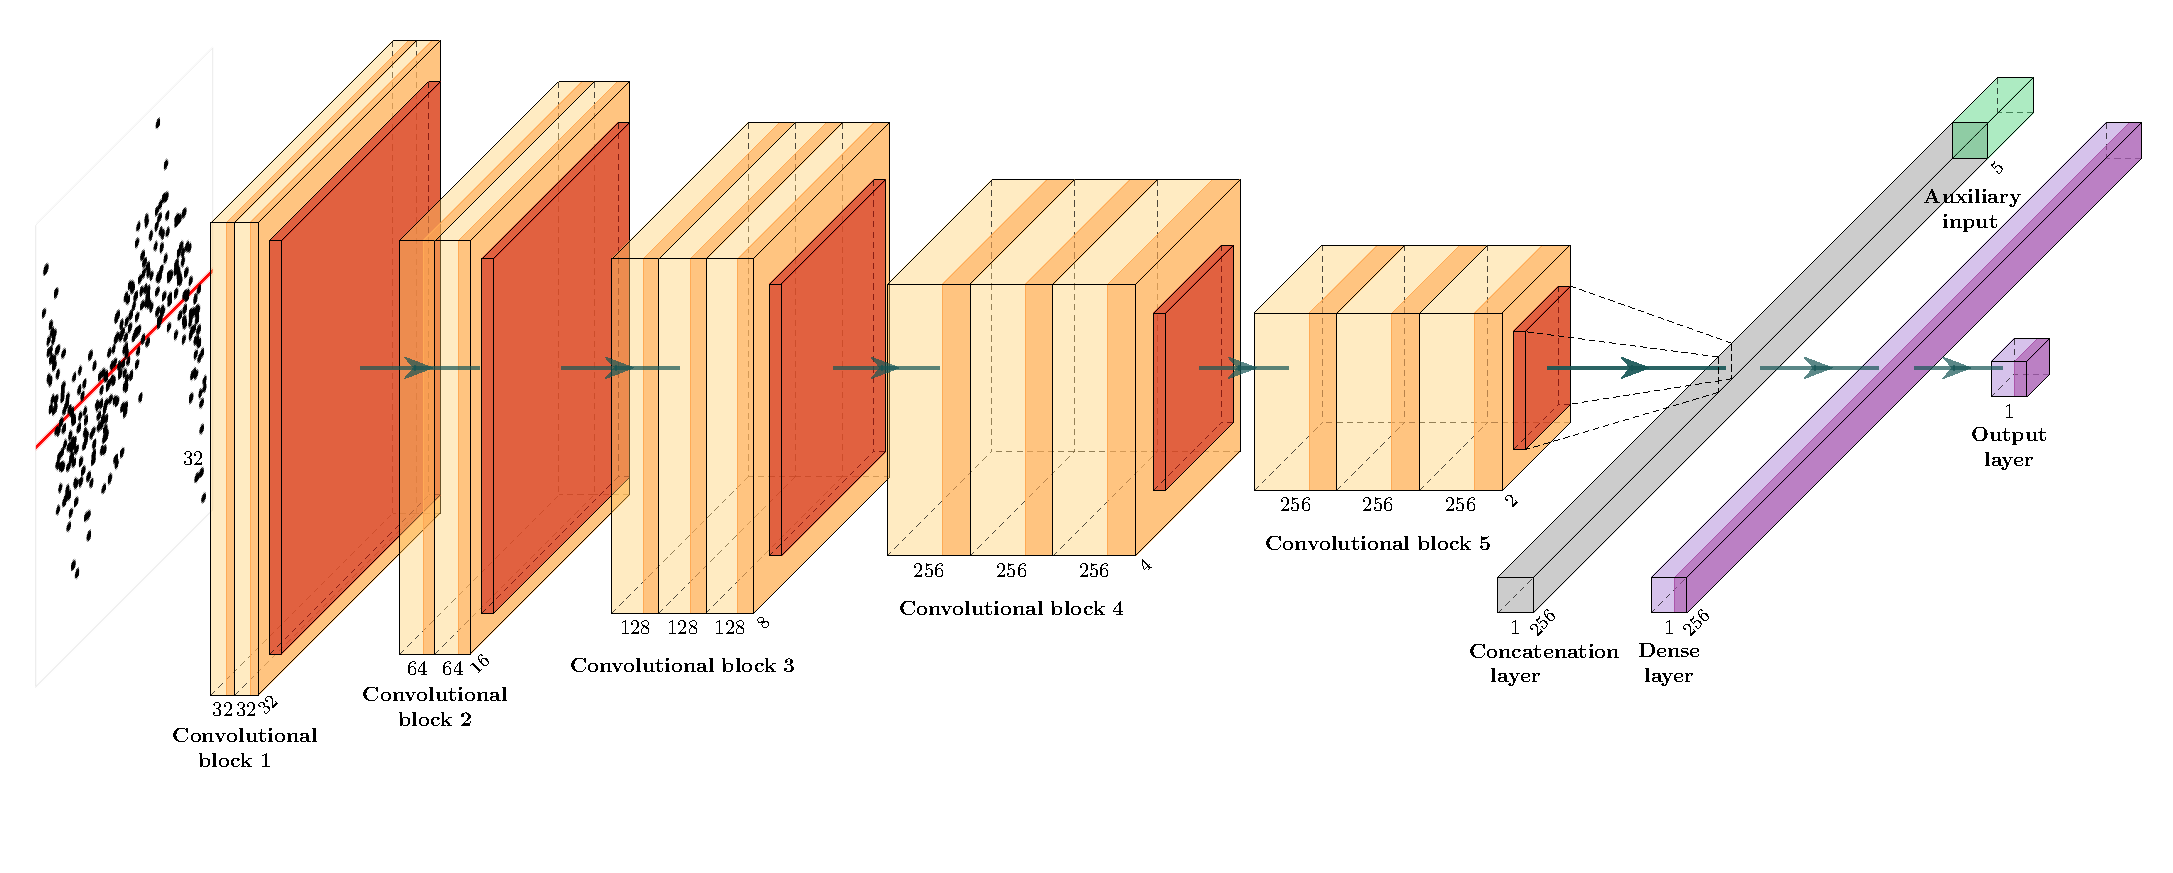
\includegraphics[width=1\linewidth]{figures/cnn} 

}

\caption{Diagram of the architecture of the optimized computer vision model. Numbers at the bottom of each box show the shape of the output of each layer. The band of each box drawn in a darker color indicates the use of the rectified linear unit activation function.  Yellow boxes are 2D convolutional layers, orange boxes are pooling layers, the grey box is the concatenation layer, and the purple boxes are dense layers.}\label{fig:cnn-diag}
\end{figure}

The model \DIFdelbegin \DIFdel{begins with an input layer of shape
\(n \times h \times w \times 3\), capable of
handling \(n\) RGB images. This is followed by a grayscale conversion layer using the luma formula
under the }\DIFdelend \DIFaddbegin \DIFadd{accepts residual plots rendered as \(h \times w\) RGB images,
with \(h,w \in \{32, 64, 128\}\), allowing us to study the effect of
image resolution on predictive performance while balancing computational
cost. Images are first converted to grayscale using the }\DIFaddend Rec. 601 \DIFdelbegin \DIFdel{standard \mbox{%DIFAUXCMD
\citep{series2011studio}}\hskip0pt%DIFAUXCMD
, which converts the color image to grayscale. Grayscale suffices for our task since }\DIFdelend \DIFaddbegin \DIFadd{luma
formula \mbox{%DIFAUXCMD
\citep{series2011studio}}\hskip0pt%DIFAUXCMD
, as the }\DIFaddend data points are plotted in
black \DIFaddbegin \DIFadd{on a white background. The background also includes a red
reference line at \(y = 0\), which is preserved under this conversion}\DIFaddend .
\DIFdelbegin \DIFdel{We experiment with three combinations of
\(h\) and \(w\): \(32 \times 32\), \(64 \times 64\), and
\(128 \times 128\), aiming to achieve sufficiently high image resolution
for the problem at hand.
}\DIFdelend 

The processed \DIFdelbegin \DIFdel{image is used as the input for }\DIFdelend \DIFaddbegin \DIFadd{images are used as input to }\DIFaddend the first convolutional block.
The model \DIFdelbegin \DIFdel{comprises at most }\DIFdelend \DIFaddbegin \DIFadd{consists of up to }\DIFaddend five consecutive convolutional blocks,
mirroring the original VGG16 architecture. Within each block, \DIFdelbegin \DIFdel{there are two
2D convolutional layers followed by two activation layers,
respectively. Subsequently, a 2D }\DIFdelend \DIFaddbegin \DIFadd{two
\(3 \times 3\) convolutional layers are applied, each followed by batch
normalization for training stability and a rectified linear unit (ReLU)
activation for non-linearity. The block concludes with a \(2 \times 2\)
}\DIFaddend max-pooling \DIFdelbegin \DIFdel{layer follows the second
activation layer. The 2D convolutional layer convolves the input with a fixed number of \(3 \times 3\) convolution filters, while the 2D
max-pooling }\DIFdelend layer \DIFdelbegin \DIFdel{downsamples the input along its }\DIFdelend \DIFaddbegin \DIFadd{that downsamples the }\DIFaddend spatial dimensions by taking the
maximum \DIFdelbegin \DIFdel{value over a \(2 \times 2\) window }\DIFdelend \DIFaddbegin \DIFadd{over non-overlapping windows }\DIFaddend for each channel\DIFdelbegin \DIFdel{of the input. The activation layer employs the rectified linear unit
(ReLU) activation function, a standard practice in deep learning, which
introduces a non-linear transformation of the output of the 2D
convolutional layer. Additionally, to regularize training, a batch
normalization layer is added after each 2D convolutional layer and
before the activation layer. Finally, a }\DIFdelend \DIFaddbegin \DIFadd{. A }\DIFaddend dropout layer
is \DIFdelbegin \DIFdel{appended }\DIFdelend \DIFaddbegin \DIFadd{then applied }\DIFaddend at the end of each \DIFdelbegin \DIFdel{convolutional }\DIFdelend block to randomly \DIFdelbegin \DIFdel{set some inputs to zero
}\DIFdelend \DIFaddbegin \DIFadd{deactivate
activations }\DIFaddend during training, \DIFdelbegin \DIFdel{further aiding in }\DIFdelend \DIFaddbegin \DIFadd{improving }\DIFaddend regularization.

The \DIFdelbegin \DIFdel{output of the last convolutional block is summarized by either a
}\DIFdelend \DIFaddbegin \DIFadd{final convolutional output is aggregated using either }\DIFaddend global
max-pooling \DIFdelbegin \DIFdel{layer or a }\DIFdelend \DIFaddbegin \DIFadd{or }\DIFaddend global average-pooling\DIFdelbegin \DIFdel{layer, resulting in
}\DIFdelend \DIFaddbegin \DIFadd{, producing }\DIFaddend a two-dimensional
\DIFdelbegin \DIFdel{tensor. To enrich predictions with additional
information beyond visual features, this tensor }\DIFdelend \DIFaddbegin \DIFadd{feature representation. This feature representation }\DIFaddend is concatenated with
an \DIFdelbegin \DIFdel{additional }\DIFdelend \(n \times 5\) tensor \DIFdelbegin \DIFdel{, which contains }\DIFdelend \DIFaddbegin \DIFadd{containing }\DIFaddend the ``Monotonic'', ``Sparse'',
``Splines'', and ``Striped'' measures computed using the
\texttt{cassowaryr} R package \citep{mason2022cassowaryr}, along with
the \DIFdelbegin \DIFdel{number of observations for \(n\) residual plots. These measures were
selected for their reliability and efficiency, as other scagnostics
occasionally caused R process crashes (\(\sim 5\%\)) during data
preparation due to a bug in the }\texttt{\DIFdel{interp}} %DIFAUXCMD
\DIFdel{package
\mbox{%DIFAUXCMD
\citep{Albrecht2023interp}}\hskip0pt%DIFAUXCMD
. Although this bug was later fixed at our
request, the fix came too late to re-train the model. Moreover, their
high computational cost makes them unsuitable for fast inference.
}\DIFdelend \DIFaddbegin \DIFadd{sample size for each residual plot. }\footnote{\DIFadd{Note: These measures
  were selected for their reliability and computational efficiency.
  Other scagnostics were excluded because they occasionally caused R
  process crashes (\(\sim 5\%\)) during data preparation due to a bug in
  the }\texttt{\DIFadd{interp}} \DIFadd{package \mbox{%DIFAUXCMD
\citep{Albrecht2023interp}}\hskip0pt%DIFAUXCMD
. Although this
  issue was later fixed at our request, the corrected version was not
  available during model training, and the full set of features was also
  deemed too computationally expensive for efficient inference.}}
\DIFaddend 

The concatenated \DIFdelbegin \DIFdel{tensor is then fed into }\DIFdelend \DIFaddbegin \DIFadd{feature tensor is passed to }\DIFaddend the final prediction block\DIFdelbegin \DIFdel{.
This block }\DIFdelend \DIFaddbegin \DIFadd{,
which }\DIFaddend consists of two \DIFdelbegin \DIFdel{fully-connected }\DIFdelend \DIFaddbegin \DIFadd{fully connected }\DIFaddend layers. The first layer \DIFdelbegin \DIFdel{contains }\DIFdelend \DIFaddbegin \DIFadd{has }\DIFaddend at
least \(128\) units \DIFdelbegin \DIFdel{, followed by a dropout layer. A batch normalization layer is inserted between the fully-connected layer and the dropout
layer for regularizationpurposes}\DIFdelend \DIFaddbegin \DIFadd{and is followed by batch normalization and dropout
for regularization}\DIFaddend . The second \DIFdelbegin \DIFdel{fully-connected layer consists of only one unit, serving as the output
of the model.
}%DIFDELCMD < 

%DIFDELCMD < %%%
\DIFdel{The model weights \(\boldsymbol{\theta}\) were randomly initialized
using the Glorot Uniform method \mbox{%DIFAUXCMD
\citep{glorot2010understanding} }\hskip0pt%DIFAUXCMD
and they
were optimized by the Adam optimizer \mbox{%DIFAUXCMD
\citep{kingma2014adam} }\hskip0pt%DIFAUXCMD
with the MSE
loss function
\(\hat{\boldsymbol{\theta}} = \underset{\boldsymbol{\theta}}{\text{arg min}}\frac{1}{n_{\text{train}}}\sum_{i=1}^{n_{\text{train}}}(D_i - f_{\boldsymbol{\theta}}(V_i, S_i))^2\),
where \(n_{\text{train}}\) is the number of training samples, \(V_i\) is
the \(i\)-th residual plot and \(S_i\) is the auxiliary information
about the \(i\)-th residual plot including four scagnostics and the
number of observations}\DIFdelend \DIFaddbegin \DIFadd{fully connected layer contains a single
unit, followed by a ReLU activation to enforce non-negative outputs,
producing the final scalar prediction}\DIFaddend .

\DIFdelbegin \section{\DIFdel{Data Generation and Model
Training}}%DIFAUXCMD
\addtocounter{section}{-1}%DIFAUXCMD
\DIFdelend \DIFaddbegin \subsection{\DIFadd{Data Generation and Model
Training}}\DIFaddend \label{sec-model-data-generation}

To train the computer vision model for \DIFdelbegin \DIFdel{computing }\DIFdelend \DIFaddbegin \DIFadd{estimating }\DIFaddend \(\hat{D}\)\DIFdelbegin \DIFdel{(as
described in Section \ref{sec-model-distance-estimation}), we
used
}\DIFdelend \DIFaddbegin \DIFadd{, we
constructed a dataset of }\DIFaddend paired residual plots and their corresponding
\(D\) values. In deep learning, \DIFdelbegin \DIFdel{it is common to train computer vision models with synthetic data , especially }\DIFdelend \DIFaddbegin \DIFadd{synthetic data are commonly used for
training vision models }\DIFaddend when labelled data are scarce, costly, or
difficult to \DIFdelbegin \DIFdel{annotate }\DIFdelend \DIFaddbegin \DIFadd{obtain }\DIFaddend reliably \citep{nikolenko2021synthetic}. This \DIFdelbegin \DIFdel{approach is
particularly suitable when the underlying }\DIFdelend \DIFaddbegin \DIFadd{is
particularly appropriate when the }\DIFaddend data-generating \DIFdelbegin \DIFdel{process is well
understood and large numbers of controlled examples can be
produced, allowing the model to learn visual patterns associated with
specific violationswithout the cost and ambiguity of manual labelling}\DIFdelend \DIFaddbegin \DIFadd{mechanism is well
specified, enabling controlled generation of large-scale examples that
encode known structural violations}\DIFaddend . Accordingly, we generated \DIFdelbegin \DIFdel{a synthetic dataset consisting of }\DIFdelend 80,000
training \DIFaddbegin \DIFadd{samples }\DIFaddend and 8,000 test \DIFdelbegin \DIFdel{residual plots}\DIFdelend \DIFaddbegin \DIFadd{samples}\DIFaddend , providing full control over the
\DIFdelbegin \DIFdel{data-generating process, precise }\DIFdelend \DIFaddbegin \DIFadd{generative process, exact }\DIFaddend computation of \(D\), \DIFdelbegin \DIFdel{cost-effective
scaling, and coverage of a wide range of visual }\DIFdelend \DIFaddbegin \DIFadd{and broad coverage of
residual }\DIFaddend patterns associated with model \DIFdelbegin \DIFdel{violations}\DIFdelend \DIFaddbegin \DIFadd{misspecification}\DIFaddend .

The simulated data incorporated three common types of residual
departures: non-linearity, heteroskedasticity, and non-normality. These
\DIFdelbegin \DIFdel{were introduced }\DIFdelend \DIFaddbegin \DIFadd{effects were induced }\DIFaddend by fitting a \DIFdelbegin \DIFdel{standard }\DIFdelend simple linear regression model to data
generated from a more flexible \DIFdelbegin \DIFdel{model }\DIFdelend \DIFaddbegin \DIFadd{underlying process }\DIFaddend based on Hermite
polynomials \citep{hermite1864nouveau}, multiple predictors, and \DIFdelbegin \DIFdel{varying
distributions in both predictors and error terms}\DIFdelend \DIFaddbegin \DIFadd{a range
of predictor and error distributions}\DIFaddend . A comprehensive grid of parameter
\DIFdelbegin \DIFdel{combinations was explored to generate a wide range of
residual patterns. Importantly, the simulation included scenarios with multiple violations occurring simultaneously.
}\DIFdelend \DIFaddbegin \DIFadd{settings was used to produce diverse residual behaviours, including
configurations with multiple simultaneous violations.
}

\DIFaddend To ensure uniform coverage across the \DIFdelbegin \DIFdel{difficulty scale of the target variable }\DIFdelend \DIFaddbegin \DIFadd{target space of }\DIFaddend \(D\), \DIFdelbegin \DIFdel{a bucket
sampling scheme was used to create a balanced dataset. Samples were
iteratively simulated and accepted into }\DIFdelend \DIFaddbegin \DIFadd{we adopted
a bucketed sampling strategy. Specifically, simulated samples were
iteratively generated and assigned to }\DIFaddend one of 50 \DIFdelbegin \DIFdel{buckets, each
representing a distinct range }\DIFdelend \DIFaddbegin \DIFadd{bins corresponding to
quantiles }\DIFaddend of \(D\)\DIFaddbegin \DIFadd{, with acceptance controlled to balance representation
across difficulty levels}\DIFaddend . Table \ref{tab:data-overall} \DIFdelbegin \DIFdel{summarizes the
number of training and test samples under the different
violation scenarios}\DIFdelend \DIFaddbegin \DIFadd{summarises the
resulting sample sizes for each violation scenario}\DIFaddend .

\begin{table}
\centering
\caption{\label{tab:data-overall}Number of training and test samples for each model violation scenario, including cases with multiple simultaneous violations. Each sample consists of a residual plot as input and the corresponding distance $D$ as the target. Root mean square error (RMSE) values for the training and test sets are shown for each scenario. Details of the synthetic data generating process used to construct these samples are provided in Appendix A.}
\centering
\resizebox{\ifdim\width>\linewidth\linewidth\else\width\fi}{!}{
\begin{tabular}[t]{lrrlr}
\toprule
\multicolumn{1}{c}{ } & \multicolumn{2}{c}{Train} & \multicolumn{2}{c}{Test} \\
\cmidrule(l{3pt}r{3pt}){2-3} \cmidrule(l{3pt}r{3pt}){4-5}
Violations & \#samples & RMSE & \#samples & RMSE\\
\midrule
no violations & 1,546 & 1.149 & 155 & 1.267\\
non-linearity & 22,184 & 0.625 & 2,218 & 0.787\\
heteroskedasticity & 10,826 & 0.528 & 1,067 & 0.602\\
non-linearity + heteroskedasticity & 10,221 & 0.593 & 985 & 0.751\\
non-normality & 10,797 & 0.279 & 1,111 & 0.320\\
non-linearity + non-normality & 8,835 & 0.472 & 928 & 0.600\\
heteroskedasticity + non-normality & 7,870 & 0.354 & 819 & 0.489\\
non-linearity + heteroskedasticity + non-normality & 7,721 & 0.432 & 717 & 0.620\\
\bottomrule
\end{tabular}}
\end{table}

\DIFdelbegin \DIFdel{The computer vision model }\DIFdelend \DIFaddbegin \DIFadd{Computer vision model parameters \(\boldsymbol{\theta}\) were randomly
initialized using the Glorot Uniform method
\mbox{%DIFAUXCMD
\citep{glorot2010understanding} }\hskip0pt%DIFAUXCMD
and optimized with the Adam optimizer
\mbox{%DIFAUXCMD
\citep{kingma2014adam} }\hskip0pt%DIFAUXCMD
under a mean squared error objective:
}\[\DIFadd{\hat{\boldsymbol{\theta}} = \underset{\boldsymbol{\theta}}{\text{arg min}}\frac{1}{n_{\text{train}}}\sum_{i=1}^{n_{\text{train}}}(D_i - f_{\boldsymbol{\theta}}(V_i, \boldsymbol{s}_i))^2,}\]
\noindent \DIFadd{where \(n_{\text{train}}\) denotes the number of training
samples, \(V_i\) is the \(i\)-th residual plot, and \(\boldsymbol{s}_i\)
represents the auxiliary tabular features, including four scagnostics
measures and sample size.
}

\DIFadd{The model }\DIFaddend was trained on paired \DIFdelbegin \DIFdel{data consisting of an
}\DIFdelend \DIFaddbegin \DIFadd{inputs consisting of }\DIFaddend RGB residual plot
\DIFdelbegin \DIFdel{image as input and the corresponding target value
}\DIFdelend \DIFaddbegin \DIFadd{images and corresponding }\DIFaddend \(D\) \DIFaddbegin \DIFadd{values}\DIFaddend , with the objective of learning
\DIFdelbegin \DIFdel{to predict \(\hat{D}\).
Model
training }\DIFdelend \DIFaddbegin \DIFadd{the mapping \(\hat{D} = f_{\boldsymbol{\theta}}(V, \boldsymbol{s})\).
Training }\DIFaddend was conducted on the MASSIVE M3 high-performance computing
platform \citep{goscinski2014multi} using TensorFlow
\citep{abadi2016tensorflow} and Keras \citep{chollet2015keras}.
Hyperparameters were \DIFdelbegin \DIFdel{optimized via Bayesian tuning with }\DIFdelend \DIFaddbegin \DIFadd{tuned using Bayesian optimisation via }\DIFaddend KerasTuner
\citep{omalley2019kerastuner}, minimizing validation root mean square
error (RMSE) \DIFdelbegin \DIFdel{across }\DIFdelend \DIFaddbegin \DIFadd{over }\DIFaddend 100 trials. The \DIFdelbegin \DIFdel{tuning process included early
stopping and considered }\DIFdelend \DIFaddbegin \DIFadd{search space included }\DIFaddend dropout rate,
batch normalization \DIFaddbegin \DIFadd{configuration}\DIFaddend , input resolution, and \DIFdelbegin \DIFdel{auxiliary inputs}\DIFdelend \DIFaddbegin \DIFadd{the inclusion
of auxiliary features}\DIFaddend .

Further details \DIFdelbegin \DIFdel{, including mathematical formulations of the synthetic data model, parameter
specifications}\DIFdelend \DIFaddbegin \DIFadd{on the synthetic data-generating process, parameter
settings}\DIFaddend , sampling scheme, example residual plots\DIFdelbegin \DIFdel{and hyperparameter tuning configuration , }\DIFdelend \DIFaddbegin \DIFadd{, and hyperparameter
search configuration }\DIFaddend are provided in \DIFdelbegin \DIFdel{the
}\DIFdelend Appendix A and \DIFaddbegin \DIFadd{Appendix }\DIFaddend C.

\DIFaddbegin \section{\DIFadd{Statistical Testing}}\label{sec-model-statistical-testing}

\DIFadd{Under the null hypothesis \(H_0\), corresponding to a correctly
specified model, the distance satisfies \(D = 0\) because \(P = Q\). In
practice, however, the estimated distance \(\hat{D}\) is generally
non-zero, even for null plots, due to sampling variability and
imperfections in the computer vision model. Consequently, statistical
significance should be assessed relative to the distribution of
estimated distances obtained from null plots rather than by the
magnitude of \(\hat{D}\) alone.
}

\DIFadd{To calibrate \(\hat{D}\), we adopt the residual rotation procedure used
for null plot generation in \mbox{%DIFAUXCMD
\citet{buja2009statistical}}\hskip0pt%DIFAUXCMD
. This involves
drawing an auxiliary response \(\boldsymbol{w}\) from
\(\mathcal{N}(\boldsymbol{0}_n, \mathbf{I}_n)\) and compute the
projected residuals
\(\hat{\boldsymbol{e}}_w = \boldsymbol{R}\boldsymbol{w}\). These are
then rescaled to match the Euclidean norm of the observed residuals,
\(\tilde{\boldsymbol{e}}_w = \hat{\boldsymbol{e}}_w \cdot \frac{\|\hat{\boldsymbol{e}}\|}{\|\hat{\boldsymbol{e}}_w\|},\)
so that \(\|\tilde{\boldsymbol{e}}_w\| = \|\hat{\boldsymbol{e}}\|\). A
null plot is then the scatter plot of
\((\hat{\boldsymbol{y}},\, \tilde{\boldsymbol{e}}_w)\), which under the
null hypothesis of a correctly specified model is statistically
indistinguishable from the true residual plot
\((\hat{\boldsymbol{y}},\, \hat{\boldsymbol{e}})\).
}

\DIFadd{Let \(\hat{D}\) denote the estimated distance for the true residual plot
and let \(\{\hat{D}_{null}^{(i)}\}_{i=1}^{m}\) denote the estimated
distances for \(m\) null plots generated under \(H_0\). For a lineup
containing \(m + 1\) plots (one true plot and \(m\) null plots), the
visual inference decision rule is
}\[\DIFadd{\text{Reject } H_0 \quad \Longleftrightarrow \quad \hat{D} > \max_{1\le i\le m} \hat{D}_{null}^{(i)}.}\]
\DIFadd{This corresponds to the standard lineup protocol, where the true
residual plot must be identified as the most visually distinct plot.
}

\DIFadd{More generally, the empirical distribution of
\(\{\hat{D}_{null}^{(i)}\}_{i=1}^{m}\) provides an estimate of the null
distribution of the test statistic. Let \(Q_{null}(\tau)\) denote the
empirical \(\tau\)-quantile of this distribution. A level-\(\alpha\)
test is then given by
}\[\DIFadd{\text{Reject } H_0 \quad \Longleftrightarrow \quad \hat{D} \ge Q_{null}(1-\alpha).}\]
\DIFadd{Equivalently, a Monte Carlo \(p\)-value can be computed as
}\[\DIFadd{\hat{p} = \frac{1}{m + 1} + \frac{1}{m + 1}\sum_{i=1}^{m} \mathbb{I}\left( \hat{D}_{null}^{(i)} \ge \hat{D} \right).}\]
\DIFadd{This is the standard simulation-based estimator of the tail probability
under \(H_0\). For computational efficiency, quantiles of the null
distribution may be pre-computed over a range of sample sizes and stored
in a lookup table, allowing approximate \(p\)-values to be obtained
without generating new null plots.
}

\section{\DIFadd{Bootstrap Variability
Assessment}}\label{sec-bootstrap-assessment}

\DIFadd{Bootstrap methods are commonly used in linear regression to assess
parameter variability without strong distributional assumptions
\mbox{%DIFAUXCMD
\citep{davison1997bootstrap, efron1994introduction}}\hskip0pt%DIFAUXCMD
. This involves
resampling the observed data (pairs of responses and predictors) with
replacement and refitting the model on each bootstrap sample.
}

\DIFadd{Similarly, this case-resampling bootstrap can be used to assess the
variability of the estimated distance \(\hat{D}\). For each bootstrap
sample \(i=1, \ldots, n_{boot}\), a regression model \(M_{boot}^{(i)}\)
is refitted using the resampled data, producing a residual plot
\(V_{boot}^{(i)}\) and a corresponding estimated distance
\(\hat{D}_{boot}^{(i)}\). The empirical distribution of
\(\{\hat{D}_{boot}^{(i)}\}_{i=1}^{n_{boot}}\) provides an estimate of
the sampling distribution of \(\hat{D}\), from which confidence
intervals may be constructed.
}

\DIFadd{More generally, each bootstrap model \(M_{boot}^{(i)}\) induces its own
null distribution of estimated distances. Let \(Q_{boot}^{(i)}(\tau)\)
denote the \(\tau\)-quantile of the corresponding null distribution. A
level-\(\alpha\) test for the \(i\)-th bootstrap model is then given by
}\[\DIFadd{\text{Reject } H_0 \quad \Longleftrightarrow \quad \hat{D}_{boot}^{(i)} \ge Q_{boot}^{(i)}(1-\alpha).}\]
\DIFadd{The proportion of bootstrap models for which \(H_0\) is rejected,
}\[\DIFadd{\frac{1}{n_{boot}}\sum_{i=1}^{n_{boot}}\mathbb{I}\left(\hat{D}_{boot}^{(i)} \ge Q_{boot}^{(i)}(1-\alpha)\right),}\]
\DIFadd{estimates how often the fitted regression model would be judged
misspecified under repeated sampling from the same data-generating
process.
}

\DIFadd{This procedure is computationally expensive because it requires
evaluating \(n_{boot}(m + 1)\) residual plots, where \(m\) denotes the
number of null plots per bootstrap sample. In practice, the
bootstrap-specific critical values \(Q_{boot}^{(i)}(1-\alpha)\) may be
approximated by the corresponding quantile \(Q_{null}(1-\alpha)\) from
the original null distribution, substantially reducing the computational
burden.
}

\DIFaddend \section{Results}\label{sec-model-results}

\subsection{Model Performance}\label{model-performance}

Table \ref{tab:performance} summarizes the test performance of \DIFdelbegin \DIFdel{optimized
models using }\DIFdelend \DIFaddbegin \DIFadd{the
optimized models across }\DIFaddend three input sizes\DIFaddbegin \DIFadd{, using 80,000 training samples
and 8,000 test samples generated as described in Section
\ref{sec-model-data-generation}}\DIFaddend . The \(32 \times 32\) model consistently
outperformed others, with a mean absolute error of approximately
\(0.43\), a negligible deviation given the typical \(D\) range of \(0\)
to \(7\). High \(R^2\) values also indicated strong linear correlation
between predictions and targets. Based on these results, we used the
best-performing \(32 \times 32\) model for subsequent analyses.

Figure \ref{fig:model-performance} shows a hexagonal heatmap of
\(D - \hat{D}\) versus \(D\). Smoothing curves \citep[fitted by
generalized additive models,][]{hastie2017generalized} reveal that all
models performed well for \(1.5 < D < 6\), where no structural issues
were observed. Over-prediction occurred when \(D < 1.5\), and
under-prediction primarily when \(\hat{D} > 6\).

For null plots (\(D = 0\)), over-prediction was expected (see Section
\DIFdelbegin \DIFdel{\ref{sec-model-lineup-evaluation}}\DIFdelend \DIFaddbegin \DIFadd{\ref{sec-model-statistical-testing}}\DIFaddend ), but not under-prediction.
Therefore, we analysed the relationship between residuals and all the
factors involved in the data generating process. We found that most
deviations stemmed from non-linearity and the presence of a second
predictor in the synthetic data model, where small \DIFdelbegin \DIFdel{\(\varepsilon\) }\DIFdelend \DIFaddbegin \DIFadd{error }\DIFaddend variances
caused under-predictions and large \DIFdelbegin \DIFdel{\(\varepsilon\) }\DIFdelend \DIFaddbegin \DIFadd{error }\DIFaddend variances caused
over-prediction, as illustrated in Figure \ref{fig:over-under}.

To investigate further, we stratified the train and test set by
violation type and re-evaluated performance (Table
\ref{tab:data-overall}). It was found that null plots had the poorest
metrics, while non-normality cases were easiest to predict, with RMSE
around \(0.3\). Non-linearity (\(\text{RMSE} \approx  0.8\)) was harder
to assess than heteroskedasticity (\(\text{RMSE} \approx  0.6\)) or
non-normality (\(\text{RMSE} \approx  0.3\)). Plots with multiple
violations showed intermediate performance.

\begin{table}

\caption{\label{tab:performance}The test performance of three optimized models with different input sizes. The metrics are computed by comparing the estimated distance $\hat{D}$ (model output) and the target distance $D$ generated from the synthetic data model. RMSE represents the root mean squared error; $R^2$ is the squared correlation between the two quantities; MAE denotes the mean absolute error; and Huber loss refers to the average Huber loss computed over the test set.}
\centering
\begin{tabular}[t]{lrrrr}
\toprule
 & RMSE & $R^2$ & MAE & Huber loss\\
\midrule
$32 \times 32$ & 0.660 & 0.901 & 0.434 & 0.18\\
$64 \times 64$ & 0.674 & 0.897 & 0.438 & 0.19\\
$128 \times 128$ & 0.692 & 0.892 & 0.460 & 0.20\\
\bottomrule
\end{tabular}
\end{table}

\begin{figure}[!h]

{\centering 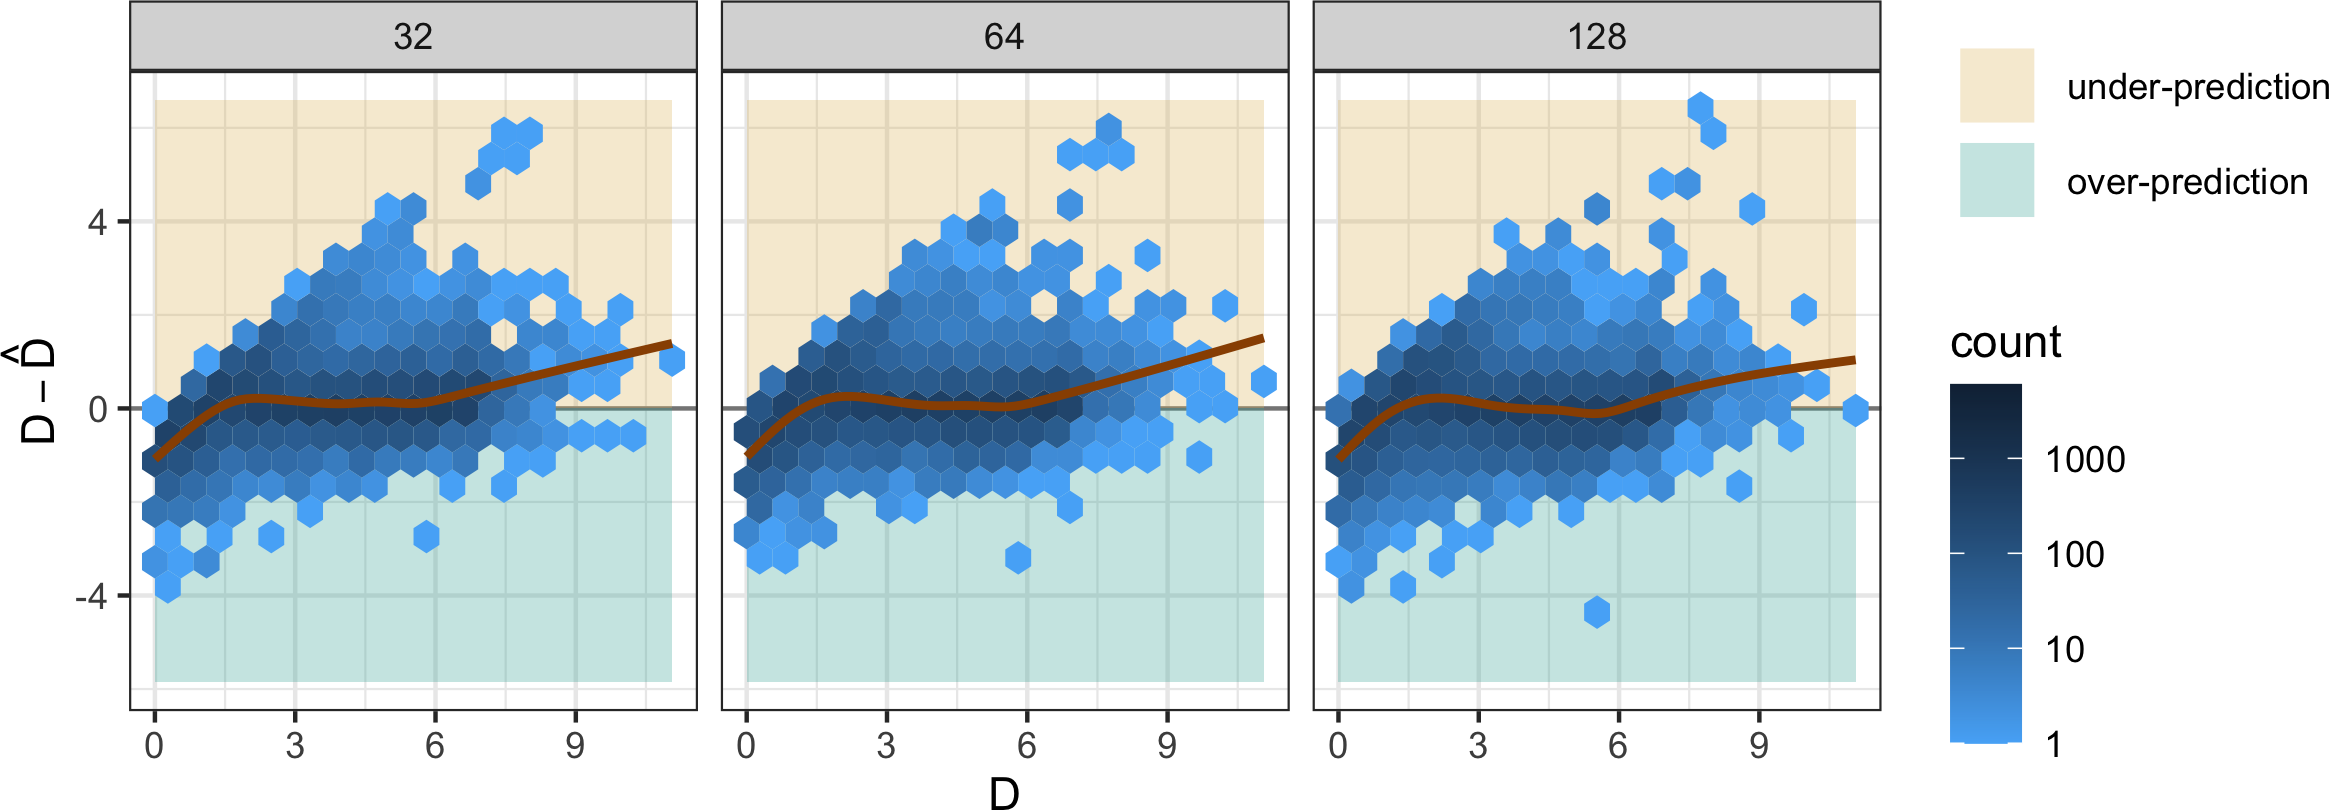
\includegraphics[width=1\linewidth]{paper_files/figure-latex/model-performance-1} 

}

\caption{Hexagonal heatmap for difference in $D$ and $\hat{D}$ vs $D$ on test data for three optimized models with different input sizes. The brown lines are smoothing curves produced by fitting generalized additive models. Over-prediction and under-prediction can be observed for small $D$ and large $D$ respectively.}\label{fig:model-performance}
\end{figure}

\begin{figure}[!h]

{\centering 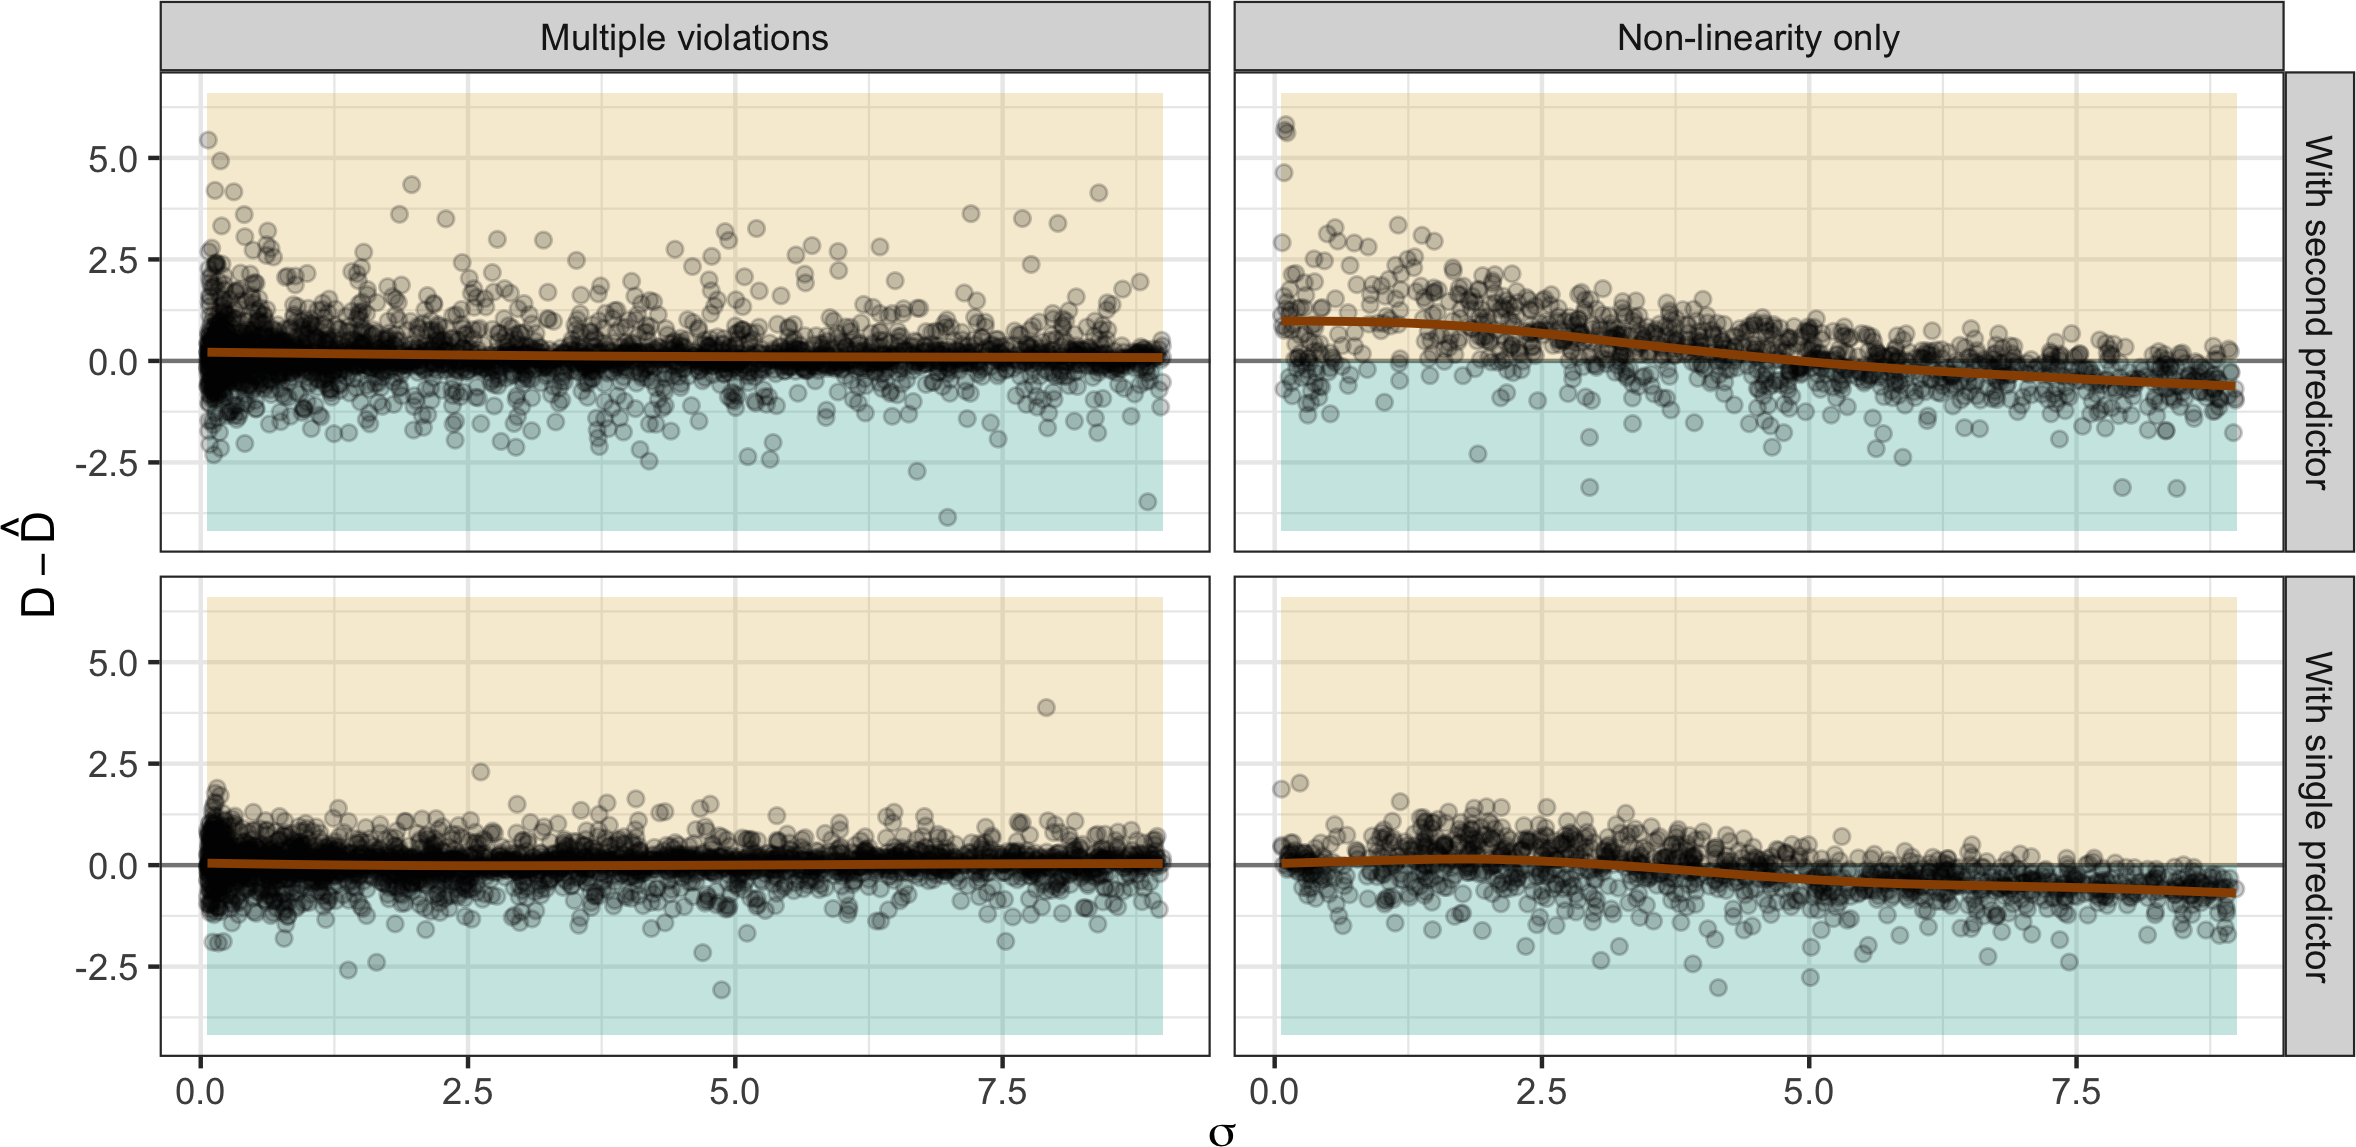
\includegraphics[width=1\linewidth]{paper_files/figure-latex/over-under-1} 

}

\caption{Scatter plots for difference in $D$ and $\hat{D}$ vs $\sigma$ on test data for the $32 \times 32$ optimized model. The data is grouped by whether the regression has only non-linearity violation, and whether it includes a second predictor in the regression formula. The brown lines are smoothing curves produced by fitting generalized additive models. Under-prediction mainly occurs when the data-generating process has small $\sigma$, a second predictor, and only non-linearity as the model violation.}\label{fig:over-under}
\end{figure}

\subsection{Comparison with Human Visual Inference and Conventional
Tests}\label{comparison-with-human-visual-inference-and-conventional-tests}

\subsubsection{Overview of the Human Subject
Experiment}\label{overview-of-the-human-subject-experiment}

In order to check the validity of the proposed computer vision model,
residual plots presented in the human subject experiment conducted by
\citet{li2024plot} \DIFdelbegin \DIFdel{will be assessed. }%DIFDELCMD < 

%DIFDELCMD < %%%
\DIFdel{This study has }\DIFdelend \DIFaddbegin \DIFadd{was assessed. The study }\DIFaddend collected 7,974 \DIFdelbegin \DIFdel{human responses
to }\DIFdelend \DIFaddbegin \DIFadd{responses
across }\DIFaddend 1,152 lineups\DIFdelbegin \DIFdel{. Each
lineup contains one randomly placed }\DIFdelend \DIFaddbegin \DIFadd{, each containing one randomly positioned }\DIFaddend true
residual plot and 19 null plots. \DIFdelbegin \DIFdel{Among the 1, 152 lineups, }\DIFdelend \DIFaddbegin \DIFadd{Of these, }\DIFaddend 24 \DIFdelbegin \DIFdel{are attention check lineups in which
the visual patterns are designed to be extremely obvious and very
different from the corresponding to null plots}\DIFdelend \DIFaddbegin \DIFadd{were attention-check
lineups with highly obvious patterns}\DIFaddend , 36 \DIFdelbegin \DIFdel{are null lineups where all the lineups consist of }\DIFdelend \DIFaddbegin \DIFadd{were null lineups containing
}\DIFaddend only null plots, 279 \DIFdelbegin \DIFdel{are lineups with
uniform predictor distribution }\DIFdelend \DIFaddbegin \DIFadd{involved uniformly distributed predictors and were
}\DIFaddend evaluated by 11 participants \DIFaddbegin \DIFadd{each}\DIFaddend , and the remaining 813 \DIFdelbegin \DIFdel{are lineups with }\DIFdelend \DIFaddbegin \DIFadd{involved
}\DIFaddend discrete, skewed\DIFdelbegin \DIFdel{or normal predictor
distribution }\DIFdelend \DIFaddbegin \DIFadd{, or normally distributed predictors and were }\DIFaddend evaluated
by 5 participants \DIFdelbegin \DIFdel{. Attention check lineups }\DIFdelend \DIFaddbegin \DIFadd{each. Attention-check }\DIFaddend and null lineups \DIFdelbegin \DIFdel{will not be assessed in the following }\DIFdelend \DIFaddbegin \DIFadd{are excluded
from the present }\DIFaddend analysis.

\DIFdelbegin \DIFdel{In \mbox{%DIFAUXCMD
\citet{li2024plot}}\hskip0pt%DIFAUXCMD
, the residual plots are simulated from a data
generating process that corresponds to a }\DIFdelend \DIFaddbegin \DIFadd{Participants were recruited through Prolific. Most were not experts in
residual plots, and 56.7\% reported no prior experience with studies
involving data visualisations. The sample was approximately
gender-balanced, more than half held a diploma or bachelor's degree, and
almost all participants were between 18 and 39 years of age.
Consequently, the results primarily reflect the ability of non-experts
to distinguish true residual plots from null plots based on visual
differences rather than specialised statistical training.
}

\DIFadd{The residual plots in \mbox{%DIFAUXCMD
\citet{li2024plot} }\hskip0pt%DIFAUXCMD
were generated from a }\DIFaddend special
case of the synthetic data model used in this study. \DIFdelbegin \DIFdel{A key feature of the design is that model
violations
are }\DIFdelend \DIFaddbegin \DIFadd{Model violations
were }\DIFaddend introduced independently, \DIFdelbegin \DIFdel{meaning }\DIFdelend \DIFaddbegin \DIFadd{so }\DIFaddend non-linearity and heteroskedasticity
\DIFdelbegin \DIFdel{do not co-exist within a single lineupbut are
instead assigned uniformly across different lineups. Moreover}\DIFdelend \DIFaddbegin \DIFadd{did not co-occur within the same lineup. In addition}\DIFaddend , the experimental
design \DIFdelbegin \DIFdel{does not account for }\DIFdelend \DIFaddbegin \DIFadd{did not consider }\DIFaddend non-normality or multiple predictors.

\subsubsection{Model Performance on the Human-evaluated
Data}\label{model-performance-on-the-human-evaluated-data}

Each lineup in \citet{li2024plot} contains one true residual plot and 19
null plots. While the true residual plot's distance \(D\) depends on the
data-generating process, null plots have \(D = 0\). We used our
optimized computer vision model to estimate \(D\) for all plots. To
ensure fair comparison, we reject \(H_0\) if the true residual plot has
the highest estimated distance. Conventional tests, including the Ramsey
RESET \citep{ramsey1969tests} for non-linearity and the Breusch-Pagan
test \citep{breusch1979simple} for heteroskedasticity, were also applied
to the same data.

Table \ref{tab:experiment-performance} reports performance metrics for
\(\hat{D}\) on true residual plots. While the performance is slightly
worse than on the test data provided in Table \ref{tab:performance}, the
mean absolute error remains low and the correlation between predictions
and true values remains high. Consistent with results in Table
\ref{tab:data-overall}, non-linearity cases are harder to predict than
heteroskedasticity cases.

\begin{table}

\caption{\label{tab:experiment-performance}The performance of the $32 \times 32$ model on the data used in the human subject experiment.}
\centering
\begin{tabular}[t]{lrrrr}
\toprule
Violation & RMSE & $R^2$ & MAE & Huber loss\\
\midrule
heteroskedasticity & 0.721 & 0.852 & 0.553 & 0.235\\
non-linearity & 0.738 & 0.770 & 0.566 & 0.246\\
\bottomrule
\end{tabular}
\end{table}

\begin{table}

\caption{\label{tab:human-conv-table}Summary of the comparison of decisions made by computer vision model with decisions made by conventional tests and visual tests conducted by human.}
\centering
\begin{tabular}[t]{lrrr}
\toprule
Violations & \#Samples & \#Agreements & Agreement rate\\
\midrule
\addlinespace[0.3em]
\multicolumn{4}{l}{\textbf{Compared with conventional tests}}\\
\hspace{1em}heteroskedasticity & 540 & 464 & 0.8593\\
\hspace{1em}non-linearity & 576 & 459 & 0.7969\\
\addlinespace[0.3em]
\multicolumn{4}{l}{\textbf{Compared with visual tests conducted by human}}\\
\hspace{1em}heteroskedasticity & 540 & 367 & 0.6796\\
\hspace{1em}non-linearity & 576 & 385 & 0.6684\\
\bottomrule
\end{tabular}
\end{table}

Table \ref{tab:human-conv-table} compares the model's rejection
decisions with those of conventional tests and human visual tests.
Agreement rates are 85.95\% for heteroskedasticity cases and 79.69\% for
non-linearity cases, higher than those observed for human visual tests
(67.96\% and 66.84\%, respectively). This suggests that the model aligns
more closely with the best available conventional tests. However, as
Figure \ref{fig:conv-mosaic} shows, the model does not always reject
when conventional tests do, indicating a lower sensitivity to model
violations.

\begin{figure}[!h]

{\centering 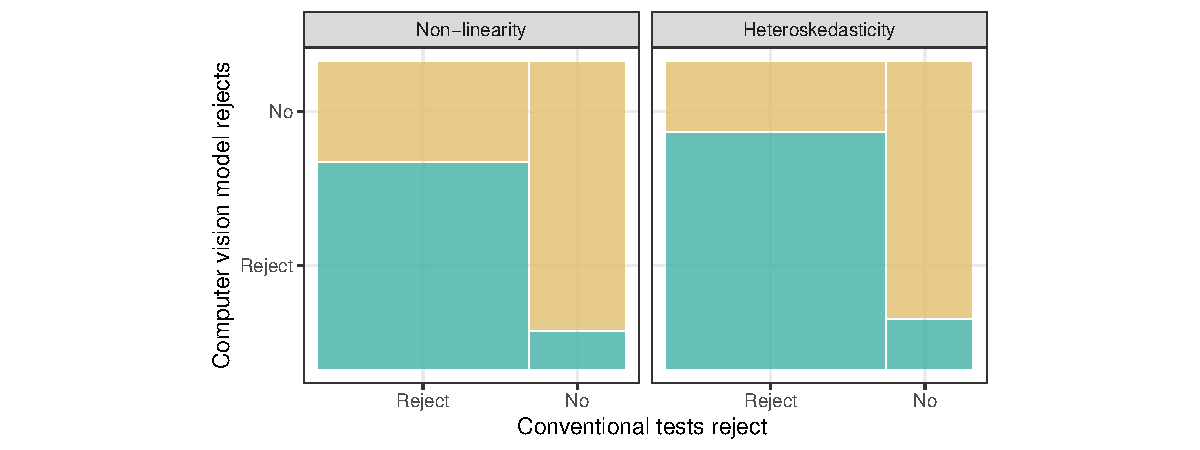
\includegraphics[width=1\linewidth]{paper_files/figure-latex/conv-mosaic-1} 

}

\caption{Rejection rate ($p$-value $\leq0.05$) of computer vision models conditional on conventional tests on non-linearity (left) and heteroskedasticity (right) lineups displayed using a mosaic plot. When the conventional test fails to reject, the computer vision mostly fails to reject the same plot as well as indicated by the height of the top right yellow rectangle, but there are non \DIFdelbeginFL \DIFdelFL{negliable }\DIFdelendFL \DIFaddbeginFL \DIFaddFL{negligible }\DIFaddendFL amount of plots where the conventional test rejects but the computer vision model fails to reject as indicated by the \DIFdelbeginFL \DIFdelFL{width }\DIFdelendFL \DIFaddbeginFL \DIFaddFL{height }\DIFaddendFL of the top left yellow rectangle.}\label{fig:conv-mosaic}
\end{figure}

To further illustrate these patterns, Figure \ref{fig:pcp} presents
parallel coordinate plots comparing decisions from human visual tests,
the computer vision model, and conventional tests. All three agree in
about 50\% of cases. When humans do not reject, conventional tests
reject in about half of those cases, whereas the model rejects in only
25\%. Notably, the model rarely rejects when both humans and
conventional tests do not, suggesting that while it is more sensitive
than humans, its rejection behavior is more aligned with human judgment
than with conventional tests.

\begin{figure}[!h]

{\centering 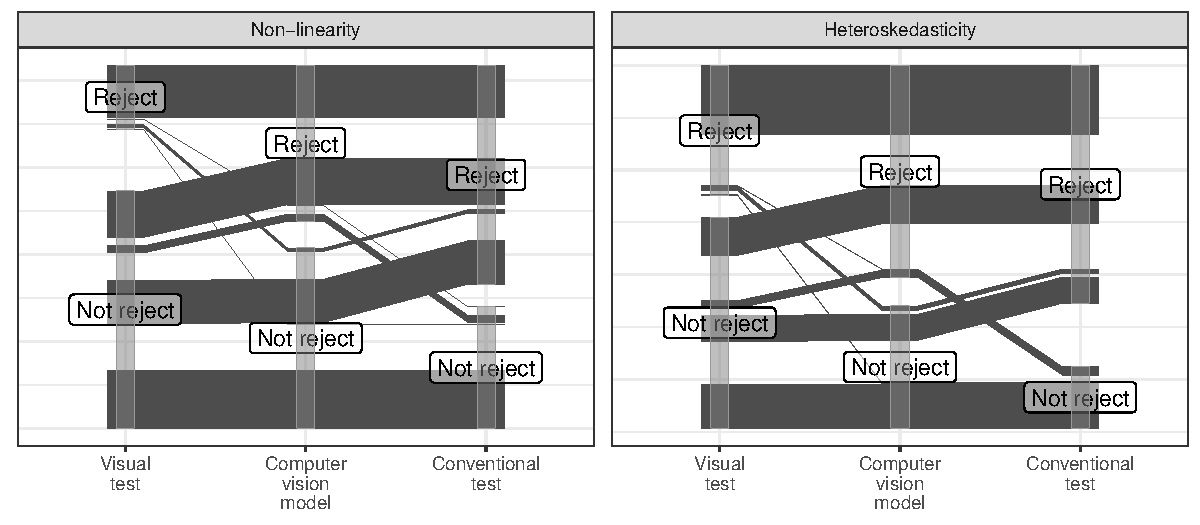
\includegraphics[width=1\linewidth]{paper_files/figure-latex/pcp-1} 

}

\caption{Parallel coordinate plots of decisions made by computer vision model, conventional tests and visual tests made by human. All three agree in around 50\% of cases. The model rejects less often than conventional tests when humans do not, and rarely rejects when both others do not, indicating closer alignment with human judgment.}\label{fig:pcp}
\end{figure}

Figure \ref{fig:power} plots rejection decisions against the true
distance \(D\). Compared to conventional tests, the computer vision
model rejects fewer cases when \(D < 4\), but a similar number of cases
when \(D > 4\). This indicates that the model is less sensitive to minor
deviations from model assumptions, while remaining comparably sensitive
to more substantial violations. Visual tests are the least sensitive
overall, showing few rejections for \(D < 2\), and requiring a higher
threshold (\(D > 5\)) for near-universal rejection, compared to
\(D > 4\) for both the model and conventional tests.

\begin{figure}[!h]

{\centering 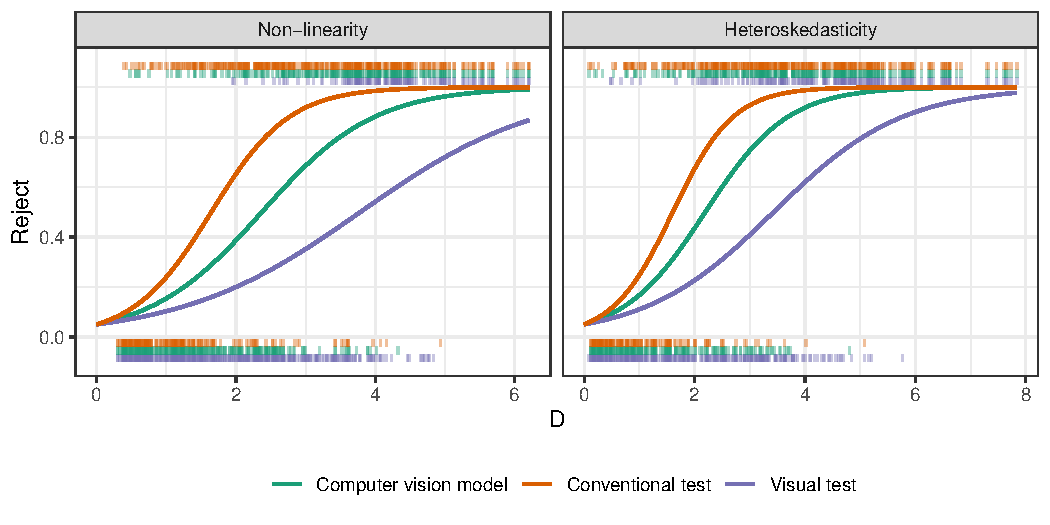
\includegraphics[width=1\linewidth]{paper_files/figure-latex/power-1} 

}

\caption{Comparison of power of visual tests, conventional tests and the computer vision model. Marks along the x-axis at the bottom of the plot represent rejections made by each type of test. Marks at the top of the plot represent acceptances. Power curves are fitted by logistic regression models with no intercept but an offset equals to $\text{log}(0.05/0.95)$. The model is less sensitive than conventional tests for small $D$ but similarly sensitive for large $D$. Visual tests are least sensitive overall. The model’s curve lies between those of conventional and visual tests.}\label{fig:power}
\end{figure}

Finally, the power curves in Figure \ref{fig:power} are fitted using
logistic regression without intercepts and with an offset of
\(\log(0.05/0.95)\) to ensure a 5\% rejection rate under \(H_0\). The
model's rejection curve consistently lies between those of conventional
and human visual tests, indicating potential to further align its
decision boundary with human visual assessment.

\subsubsection{\texorpdfstring{Adjusted
\(\delta\)-difference}{Adjusted \textbackslash delta-difference}}\label{adjusted-delta-difference}

In the experiment conducted by \citet{li2024plot}, participants could
select multiple plots per lineup. To reflect detection confidence, a
weighted detection rate was computed for each lineup: selecting zero
plots yielded a weight of 0.05; otherwise, if the true residual plot was
selected, its weight was the inverse of the number of selections.

To evaluate the proposed distance measure, we could examine the
relationship between the weighted detection rate and the
\(\delta\)-difference statistic from \citet{chowdhury2018measuring}:

\[
\delta = \bar{d}_{\text{true}} - \underset{j}{\text{max}}\left(\bar{d}_{\text{null}}^{(j)}\right) \quad \text{for}~j = 1,...,m-1,
\]

\noindent where \(\bar{d}_{\text{true}}\) is the mean distance between
the true residual plot and all null plots, and
\(\bar{d}_{\text{null}}^{(j)}\) is the mean distance from null plot
\(j\) to other nulls. These averages help address asymmetries in
pairwise distances.

However, our method only compares each plot to a theoretically ``good''
residual plot, making the original formulation inapplicable. Moreover,
since \(D_{\text{null}} = 0\) by definition and \(D\) can not be derived
from an image, we instead focus on \(\hat{D}\), the model-estimated
distance. This leads to the adjusted \(\delta\)-difference:

\[
\delta_{\text{adj}} = \hat{D} - \underset{j}{\text{max}}\left(\hat{D}_{\text{null}}^{(j)}\right) \quad \text{for}~j = 1,...,m-1,
\]

\noindent where \(\hat{D}_{\text{null}}^{(j)}\) is the estimated
distance for the \(j\)-th null plot, and \(m\) is the number of plots in
a lineup.

\begin{figure}[!h]

{\centering 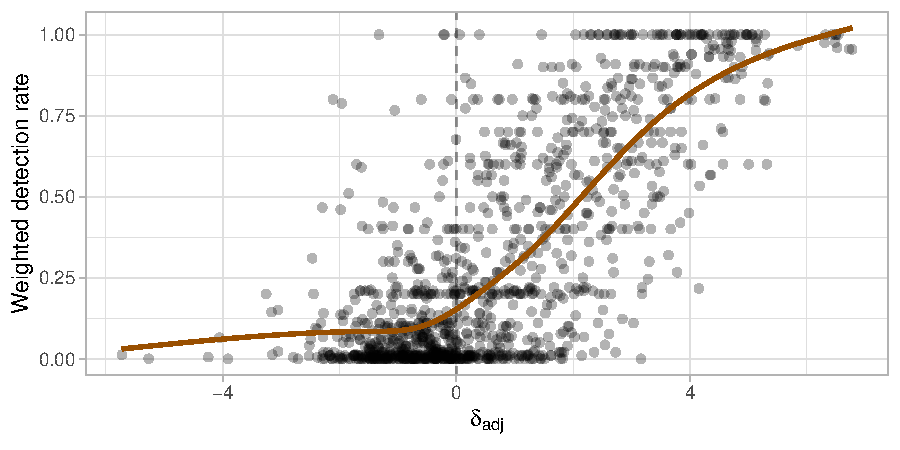
\includegraphics[width=0.8\linewidth]{paper_files/figure-latex/delta-1} 

}

\caption{A weighted detection rate vs adjusted $\delta$-difference plot. The brown line is smoothing curve produced by fitting generalized additive models. Detection generally increases with positive $\delta_{\text{adj}}$, but variability and exceptions highlight the distance measure's imperfect alignment with human perception.}\label{fig:delta}
\end{figure}

Figure \ref{fig:delta} displays the scatter plot of the weighted
detection rate against \(\delta_{\text{adj}}\). It shows that weighted
detection generally increases with \(\delta_{\text{adj}}\), especially
when it is positive. This suggests that the differences in \(\hat{D}\)
capture some aspect of the visual separability between the true and null
plots as perceived by humans, with larger positive differences generally
indicating greater distinctiveness. However, the considerable
variability in detection rates for similar \(\delta_{\text{adj}}\)
values implies that \(\hat{D}\) does not fully account for all factors
influencing human perception, and the alignment remains imperfect. A
negative \(\delta_{\text{adj}}\) suggests some null plots may appear
more visually distinctive to humans than the true residual plot. In some
instances, the weighted detection rate is close to one despite a
negative \(\delta_{\text{adj}}\). This discrepancy implies that the
distance measure may not perfectly reflect actual human behavior.

\section{Examples}\label{sec-examples}

In this section, we present the performance of the trained computer
vision model on three example datasets, including the dataset associated
with the residual plot displaying a ``left-triangle'' shape, the Boston
housing dataset \citep{harrison1978hedonic}, and the ``dino'' datasets
from the from the \texttt{datasauRus} package \citep{datasaurus}.

In the first case, both the model and human inspection correctly avoid
rejecting \(H_0\) when it is true, contrary to conventional tests,
highlighting the necessity of visual examination. The second case shows
a clear model violation detected by all tests, demonstrating the model's
practical use for less intricate tasks. The third case involves an
unusual deviation where the model and humans reject \(H_0\), but some
conventional tests do not, illustrating the benefits of visual-based
decision-making.

\subsection{Left-triangle}\label{left-triangle}

In Section \ref{sec-model-introduction}, we introduced a residual plot
(Figure \DIFdelbegin \DIFdel{\ref{fig:false-finding}}\DIFdelend \DIFaddbegin \DIFadd{\ref{fig:false-check}A}\DIFaddend ) where the ``left-triangle'' shape could
be misinterpreted as evidence of heteroskedasticity. Although the
residuals are drawn from a correctly specified model, the Breusch-Pagan
test rejects \(H_0\) (\(p = 0.046\)). This visual artifact stems from
the skewed distribution of fitted values, as \DIFaddbegin \DIFadd{later }\DIFaddend illustrated in the
lineup in Figure \ref{fig:lineup}A, where similar ``left-triangle''
patterns appear across all residual plots. Since the true plot (at
position 10) is visually indistinguishable from the null plots, a visual
test would not reject \(H_0\).

The computer vision model yields \DIFdelbegin \DIFdel{a consistent conclusion }\DIFdelend \DIFaddbegin \DIFadd{the same conclusion from the lineup}\DIFaddend . As
shown in Figure \ref{fig:false-check}\DIFaddbegin \DIFadd{C}\DIFaddend , the estimated distance
\(\hat{D}\) falls well below the 95\% quantile of the null distribution,
with a \(p\)-value of \(0.33\). The bootstrapped distribution further
suggests that rejection of the fitted model is highly unlikely.
Together, the visual and model-based tests do not reject \(H_0\), in
contrast to the Breusch-Pagan test, which lacks the context provided by
null plots and may be misled by visual artifacts.

To further interpret the model's output, the attention map in Figure
\ref{fig:false-check}B, computed as the gradient of the output with
respect to the grayscale input, shows that the top-right and
bottom-right corners of the residual plot have the most influence,
corresponding to the triangle's vertices. In addition, a principal
component analysis (PCA) of the 256 features extracted by the model's
global pooling layer (Figure \ref{fig:false-check}D) shows that null and
bootstrapped plots cluster together in the space defined by the first
two principal components, and the true residual plot is covered by the
cluster. This overlap reinforces the conclusion that the true plot is
visually indistinct, aligning with our interpretation of the lineup.

\begin{figure}[!h]

{\centering 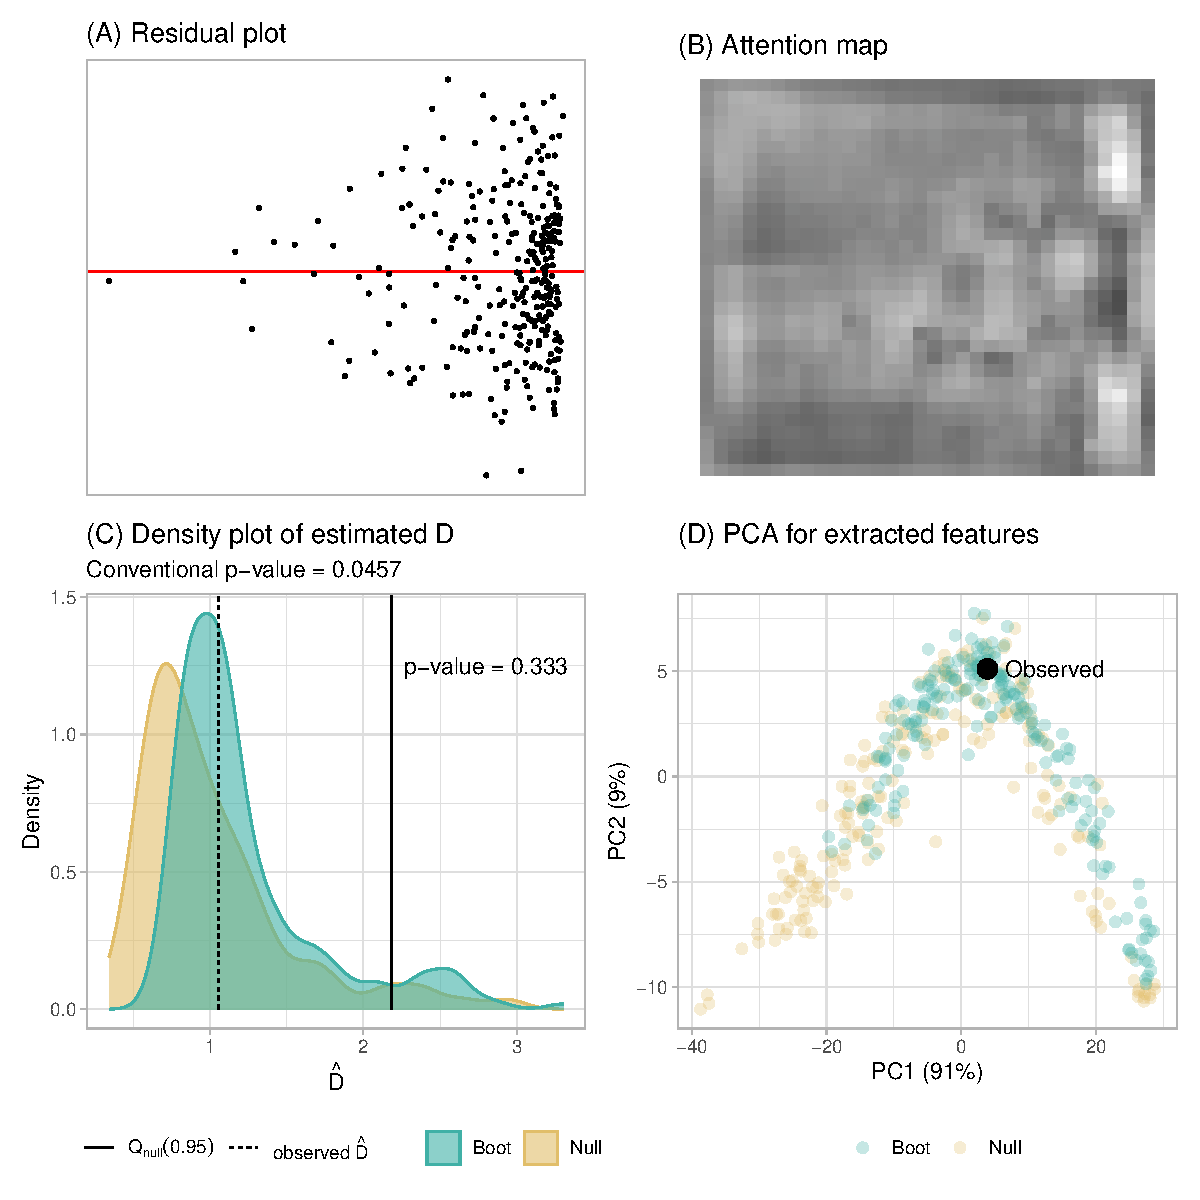
\includegraphics[width=0.8\linewidth]{paper_files/figure-latex/false-check-1} 

}

\caption{A summary of the residual plot assessment evaluated on 200 null plots and 200 bootstrapped plots. (A) The true residual plot exhibiting a \DIFdelbeginFL \DIFdelFL{"}\DIFdelendFL \DIFaddbeginFL \DIFaddFL{``}\DIFaddendFL left-triangle" shape. (B) The attention map highlights the top-right and bottom-right corners of the residual plot as the most influential.  (C) The density plot shows estimated distances for null (yellow) and bootstrapped (green) plots. The fitted model is not rejected because $\hat{D} < Q_{null}(0.95)$. (D) Null and bootstrapped plots cluster together in the space defined by the first two principal components of the global pooling layer. The cluster also covers the true residual plot.}\label{fig:false-check}
\end{figure}

\subsection{Boston Housing}\label{boston-housing}

The Boston housing dataset, originally published by
\citet{harrison1978hedonic}, provides insights into housing in the
Boston, Massachusetts area. For illustration, we use a reduced Kaggle
version containing 489 observations and four variables: average number
of rooms per dwelling (RM), percentage of lower status population
(LSTAT), pupil-teacher ratio by town (PTRATIO), and median home value
(MEDV). We fit a linear regression model with MEDV as the response and
the remaining variables as predictors, focusing on detecting
non-linearity, because the relationships between RM and MEDV or LSTAT
and MEDV are non-linear.

Figure \ref{fig:boston-check} summarizes the model evaluation. The
residual plot (Figure \ref{fig:boston-check}A) reveals a distinct
``U''-shaped pattern, suggesting non-linearity. The RESET test strongly
rejects \(H_0\) with a very small \(p\)-value, and the computer vision
model yields a large estimated distance \(\hat{D}\), well above the 95\%
quantile of the null distribution (\(p\text{-value} = 0.00498\)). The
bootstrapped distribution also shows widespread rejection, indicating
the model is likely misspecified. The attention map (Figure
\ref{fig:boston-check}B) highlights the central region of the residual
plot, corresponding to the turning point of the ``U'', as most
influential. In the PCA projection (Figure \ref{fig:boston-check}D),
bootstrapped and null plots form two distinct clusters, emphasizing the
visual separability. This aligns with the lineup in Figure
\ref{fig:lineup}B, where the true plot stands out clearly. A human
visual test would also likely reject \(H_0\) in this case.

\begin{figure}[!h]

{\centering 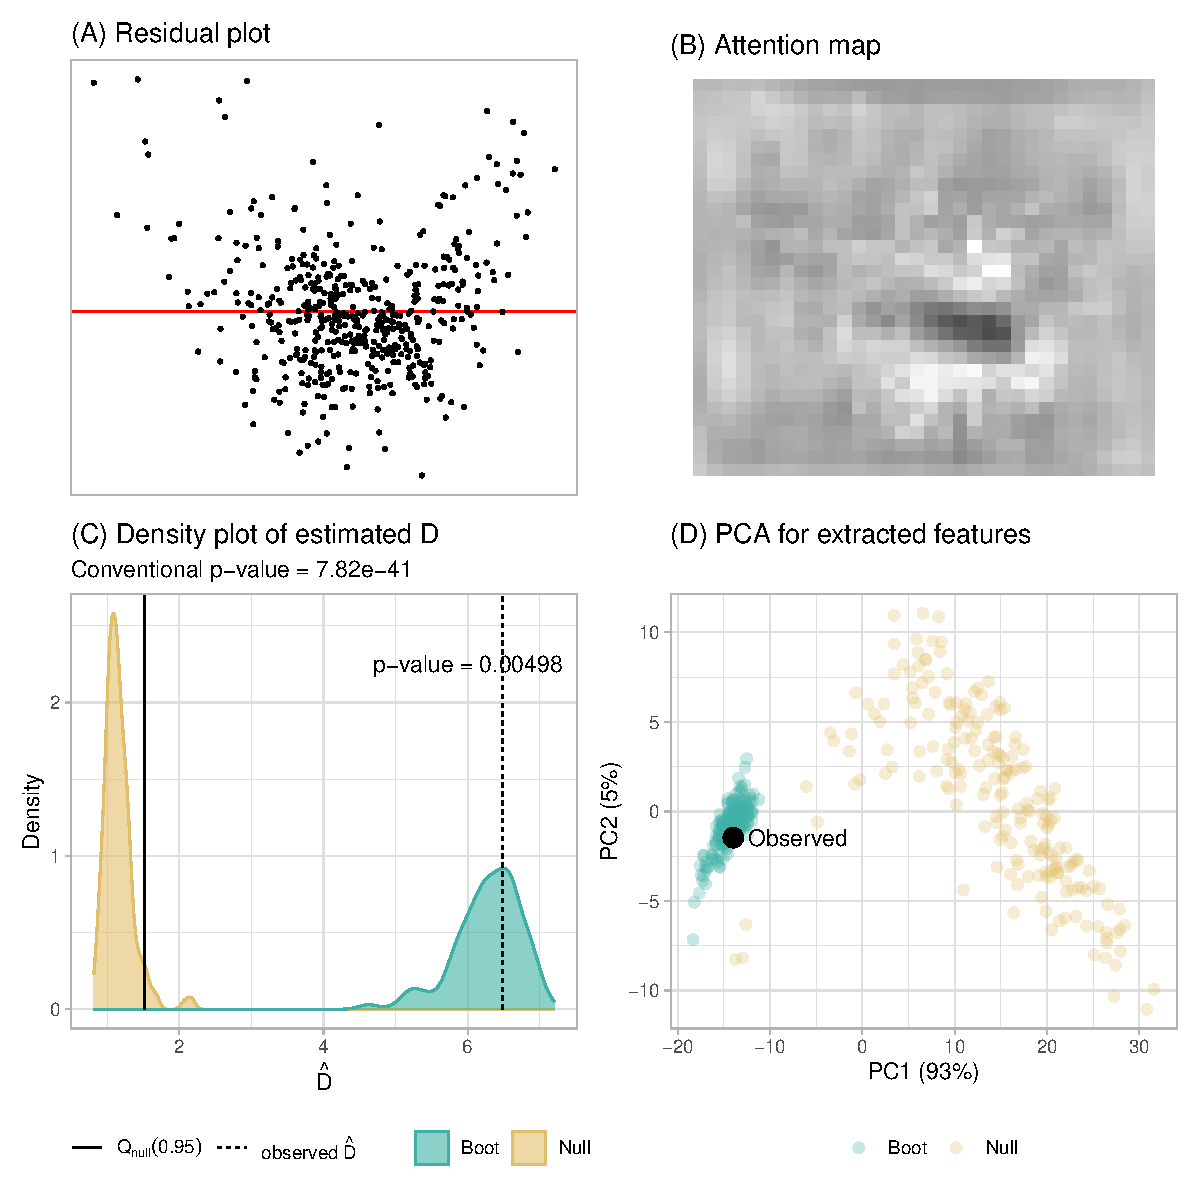
\includegraphics[width=0.8\linewidth]{paper_files/figure-latex/boston-check-1} 

}

\caption{A summary of the residual plot assessment for the Boston housing fitted model evaluated on 200 null plots and 200 bootstrapped plots. (A) The true residual plot exhibiting a \DIFdelbeginFL \DIFdelFL{"}\DIFdelendFL \DIFaddbeginFL \DIFaddFL{``}\DIFaddendFL U" shape. (B) The attention map highlights the central region of the \DIFdelbeginFL \DIFdelFL{"}\DIFdelendFL \DIFaddbeginFL \DIFaddFL{``}\DIFaddendFL U" shape as the most influential part of the residual plot. (C) The density plot shows estimated distances for null (yellow) and bootstrapped (green) plots. The fitted model is rejected because $\hat{D} \geq Q_{null}(0.95)$. (D) Bootstrapped and null plots form distinct clusters in the space of the first two principal components from the global pooling layer, highlighting their visual separability.}\label{fig:boston-check}
\end{figure}

\subsection{DatasauRus}\label{datasaurus}

Beyond detecting common issues like non-linearity, heteroskedasticity,
and non-normality, the computer vision model can also identify unusual
visual artifacts, such as shapes resembling real-world objects, as long
as such patterns do not appear in null plots. These cases are
challenging to categorize using conventional model diagnostics, so we
compare the model's output with results from the RESET test,
Breusch-Pagan test, and Shapiro-Wilk test \citep{shapiro1965analysis}.

The ``dino'' dataset from the \texttt{datasauRus} R package illustrates
this situation. It contains only two variables, \(x\) and \(y\), but
fitting a regression model produces a residual plot that clearly
resembles a dinosaur (Figure \ref{fig:dino-check}A). This pattern is
visually distinctive in the lineup shown in Figure \ref{fig:lineup}C,
where a human visual test would undoubtedly reject \(H_0\).

Consistent with this, the computer vision model assigns a distance
\(\hat{D}\) above the 95\% quantile of the null distribution
(\(p\text{-value} = 0.00498\)), leading to rejection of \(H_0\). The
bootstrapped distribution further supports this, with most fitted models
also being rejected. In contrast, the RESET and Breusch-Pagan tests
yield \(p\)-values above \(0.3\), suggesting no violation. Only the
Shapiro-Wilk test rejects normality with a small \(p\)-value.

Crucially, the attention map in Figure \ref{fig:dino-check}B highlights
the dinosaur shape, indicating that the model's decision is driven by
human-perceptible features. The model appears to capture contours and
outlines in a manner similar to human visual interpretation. In the PCA
plot (Figure \ref{fig:dino-check}D), the cluster of bootstrapped plots
is positioned at the corner of the cluster of null plots, isolated from
the cluster of null plots.

In practice, such visual artifacts would be difficult to detect without
inspecting the residual plot directly. Furthermore, analysts do not
always test for normality, and even when violations are found, they are
often deemed acceptable due to the robustness of linear regression under
quasi-likelihood theory. This example highlights the value of visual
diagnostics and the unique role of the proposed computer vision model in
supporting them.

\begin{figure}[!h]

{\centering 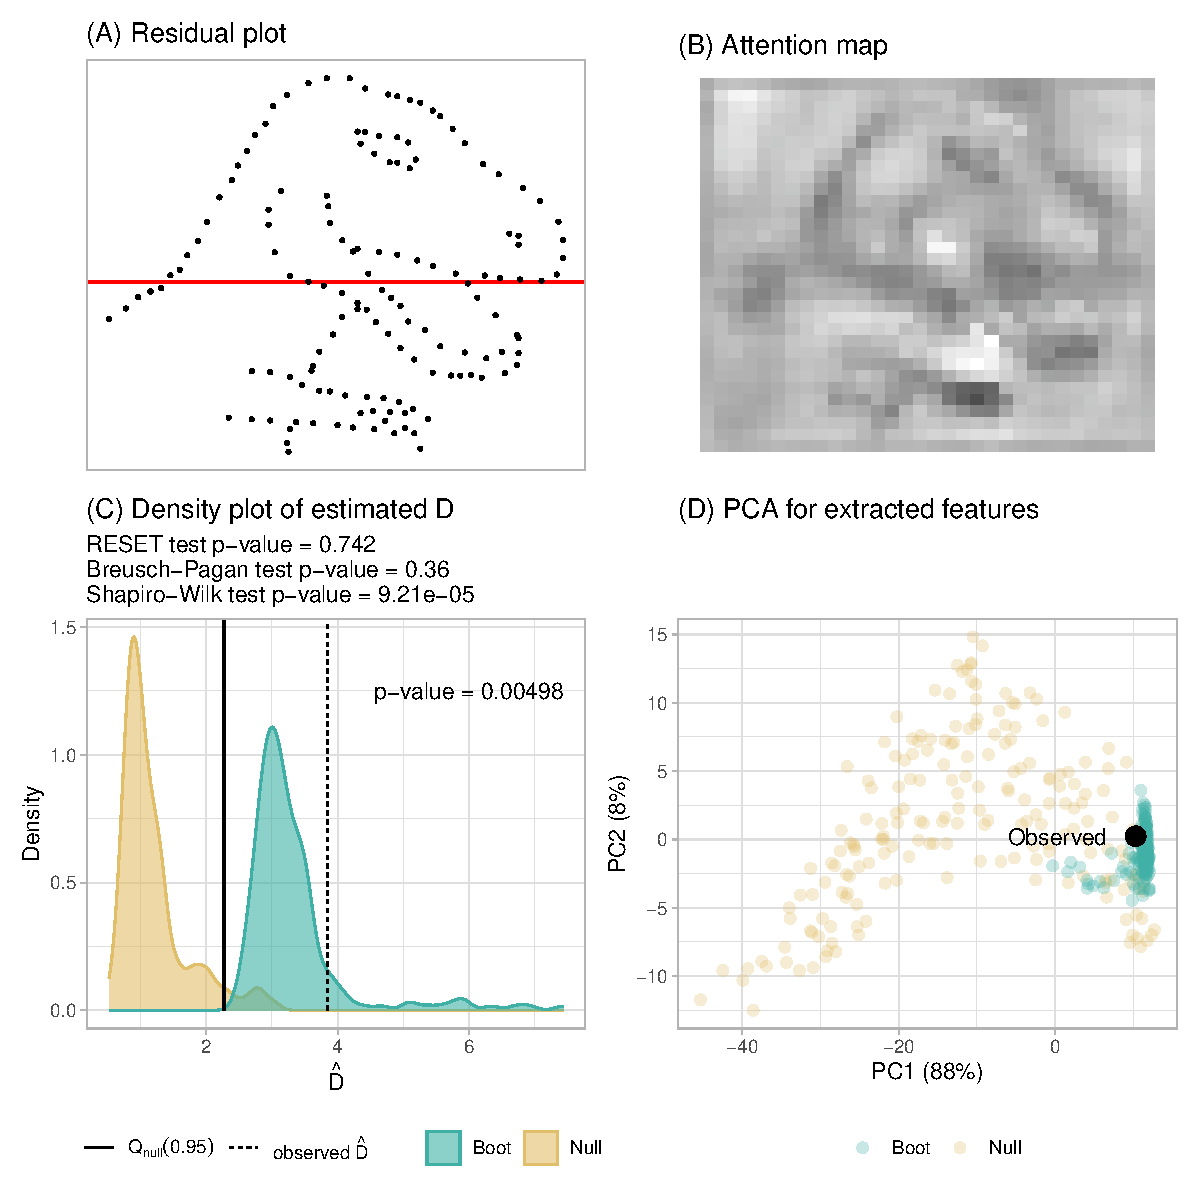
\includegraphics[width=0.8\linewidth]{paper_files/figure-latex/dino-check-1} 

}

\caption{A summary of the residual plot assessment for the datasauRus fitted model evaluated on 200 null plots and 200 bootstrapped plots. (A) The residual plot exhibits a \DIFdelbeginFL \DIFdelFL{"}\DIFdelendFL \DIFaddbeginFL \DIFaddFL{``}\DIFaddendFL dinosaur" shape. (B) The attention map highlights the \DIFaddbeginFL \DIFaddFL{``}\DIFaddendFL dinosaur\DIFaddbeginFL \DIFaddFL{" }\DIFaddendFL shape, indicating the model's decision is driven by human-recognizable features.(C) The density plot shows estimated distances for null (yellow) and bootstrapped (green) plots. The fitted model is rejected because $\hat{D} \geq Q_{null}(0.95)$. (D) The bootstrapped plots cluster at the corner of the null plot cluster, yet remain isolated in the space defined by the first two principal components of the global pooling layer.}\label{fig:dino-check}
\end{figure}

\begin{figure}[!h]

{\centering 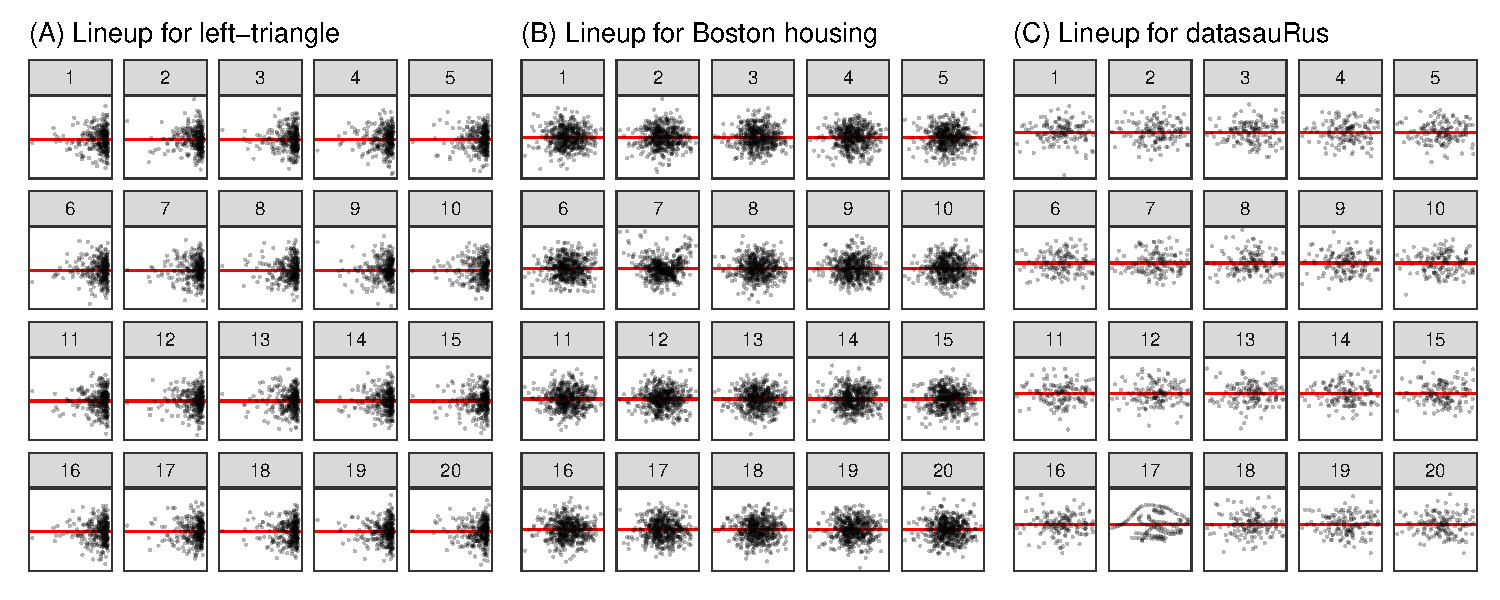
\includegraphics[width=1\linewidth]{paper_files/figure-latex/lineup-1} 

}

\caption{Lineups of residual plots for the \DIFdelbeginFL \DIFdelFL{"}\DIFdelendFL \DIFaddbeginFL \DIFaddFL{``}\DIFaddendFL left-triangle", \DIFdelbeginFL \DIFdelFL{"}\DIFdelendFL \DIFaddbeginFL \DIFaddFL{``}\DIFaddendFL Boston housing", and \DIFdelbeginFL \DIFdelFL{"}\DIFdelendFL \DIFaddbeginFL \DIFaddFL{``}\DIFaddendFL datasauRus" datasets. (A) True plot at position 10; no clear visual difference. (B) True plot at position 7; \DIFdelbeginFL \DIFdelFL{"}\DIFdelendFL \DIFaddbeginFL \DIFaddFL{``}\DIFaddendFL U"-shape clearly stands out. (C) True plot at position 17; distinctly artificial and easily identifiable.}\label{fig:lineup}
\end{figure}

\section{Limitations and Future Work}\label{limitations-and-future-work}

While the computer vision model performs well under the synthetic data
generation scheme and across the three illustrative examples, this study
has several limitations that point to directions for future work.

First, the proposed distance measure assumes the true model follows a
classical normal linear regression framework, which may be restrictive.
Although we do not explore relaxation of this assumption here, future
work could extend the approach to other types of regression models. One
possibility is to define a distance measure tailored to each model class
and re-train the computer vision model accordingly. To reduce
computational cost, the convolutional blocks from our current model
could be reused via transfer learning, as it is already effective at
capturing visual features. Alternatively, transforming residuals to
approximate normality and constant variance could allow for meaningful
comparisons under our current distance measure. However, if raw
residuals are used, the interpretation remains valid only when the
visual differences between the true and null plots are detectable by the
proposed distance measure.

Second, this study focused solely on the standard residuals vs.~fitted
values plot, leaving out other common diagnostic plots such as residuals
vs.~predictors and Q-Q plots. These alternative plots may offer
additional information and could be incorporated into a broader visual
testing framework in future research.

Finally, we chose a relatively simple computer vision architecture to
establish a baseline for automated visual inference. While the current
model shows promise, there is room to improve its alignment with human
judgment. Achieving this may require external data from surveys or
controlled experiments to better understand how human observers
interpret residual plots and how these judgments differ from the model's
outputs.

\section{Conclusions}\label{conclusions}

In this paper, we have introduced a distance measure based on the
Kullback-Leibler divergence to quantify disparity between the residual
distribution of a fitted classical normal linear regression model and
the reference distribution under correct specification. This measure
captures the extent of model violations and forms the basis of a
computer vision model that estimates the distance using residual plots
as input.

The estimated distance supports a formal statistical testing procedure
by comparing the true residual plot against null plots generated from
the fitted model. Through bootstrapping and model refitting, we also
evaluate how often a correctly specified model would be flagged as
misspecified under repeated sampling.

The trained computer vision model performs well on both training and
test data, though its performance is somewhat lower for non-linear
patterns. Statistical tests based on the model's predicted distance show
lower sensitivity than conventional tests but higher sensitivity than
human visual tests. Importantly, the predicted distance broadly aligns
with the strength of visual signals perceived by humans, though further
improvements are possible.

We demonstrate the method across several scenarios, highlighting its
effectiveness and its conceptual alignment with visual inference. Both
visual and distance-based tests act as omnibus procedures, detecting a
wide range of model violations collectively. In contrast, conventional
tests such as RESET and Breusch-Pagan target specific assumptions,
making them less flexible and potentially harder to combine without
adjusting for multiple testing.

Overall, our approach offers a practical tool to support regression
diagnostics by reducing the manual effort required for residual plot
inspection. While we recommend analysts to continue reading residual
plots whenever feasible, our method can augment the process, either as
an automated screening tool or a supplement to human judgment.

\section*{Supplementary Materials}\label{supplementary-materials}
\addcontentsline{toc}{section}{Supplementary Materials}

\begin{description}
\item{Appendix:} The appendix includes more details about the synthetic data generation process, neural network layers used in the work, model training, and model violation index. (appendix.pdf, Portable Document Format file)
\end{description}

\section*{Acknowledgement}\label{acknowledgement}
\addcontentsline{toc}{section}{Acknowledgement}

These \texttt{R} packages were used for the work: \texttt{tidyverse}
\citep{tidyverse}, \texttt{lmtest} \citep{lmtest}, \texttt{mpoly}
\citep{mpoly}, \texttt{ggmosaic} \citep{ggmosaic}, \texttt{kableExtra}
\citep{kableextra}, \texttt{patchwork} \citep{patchwork}, \texttt{glue}
\citep{glue}, \texttt{ggpcp} \citep{ggpcp}, \texttt{here} \citep{here},
and \texttt{reticulate} \citep{reticulate}.

The article was created with R packages \texttt{rticles}
\citep{rticles}, \texttt{knitr} \citep{knitr} and \texttt{rmarkdown}
\citep{rmarkdown}. The project's GitHub repository
(\url{https://github.com/TengMCing/auto_residual_reading_paper})
contains all materials required to reproduce this article.

We acknowledge the use of ChatGPT (OpenAI, GPT-4, accessed July 2025) to
improve the clarity and fluency of the manuscript text. All content was
reviewed and verified by the authors to ensure accuracy and integrity.

\section*{Data Availability
Statement}\label{data-availability-statement}
\addcontentsline{toc}{section}{Data Availability Statement}

The data that support the findings of this study are openly available in
the project's GitHub repository
(\url{https://github.com/TengMCing/auto_residual_reading_paper}).

\section*{Disclosure Statement}\label{disclosure-statement}
\addcontentsline{toc}{section}{Disclosure Statement}

No potential conflict of interest was reported by the author(s).

\bibliographystyle{tfcad}
\bibliography{bibliography.bib}





\end{document}
